%\documentclass[handout]{beamer}
\documentclass[11pt]{beamer}

\mode<presentation>
{
	\usetheme{default}
  \usecolortheme{seahorse}
  \usefonttheme{default}
	\setbeamertemplate{navigation symbols}{}
	\setbeamertemplate{caption}[numbered]
} 
\setbeamersize{text margin left=0.5cm,text margin right=0.5cm}

\usepackage{amsmath}
\usepackage{xcolor}
\usepackage{tikz}
\usepackage{tabularx}
\usepackage{listings}
\usepackage{cspsymb}
\usetikzlibrary{arrows,positioning,automata} 
\usepackage{appendixnumberbeamer}
\newcommand\todo[1]{\textcolor{red}{[#1]}}
\usepackage{pgfpages}
\newcommand*{\Scale}[2][4]{\scalebox{#1}{$#2$}} 
\usepackage{handoutWithNotes} 
\mode<handout>
{
  \usepackage{pgf}
  \usepackage{pgfpages}

\pgfpagesdeclarelayout{4 on 1 boxed}
{
  \edef\pgfpageoptionheight{\the\paperheight} 
  \edef\pgfpageoptionwidth{\the\paperwidth}
  \edef\pgfpageoptionborder{0pt}
}
{
  \pgfpagesphysicalpageoptions
  {%
    logical pages=4,%
    physical height=\pgfpageoptionheight,%
    physical width=\pgfpageoptionwidth%
  }
  \pgfpageslogicalpageoptions{1}
  {%
    border code=\pgfsetlinewidth{2pt}\pgfstroke,%
    border shrink=\pgfpageoptionborder,%
    resized width=.5\pgfphysicalwidth,%
    resized height=.5\pgfphysicalheight,%
    center=\pgfpoint{.25\pgfphysicalwidth}{.75\pgfphysicalheight}%
  }%
  \pgfpageslogicalpageoptions{2}
  {%
    border code=\pgfsetlinewidth{2pt}\pgfstroke,%
    border shrink=\pgfpageoptionborder,%
    resized width=.5\pgfphysicalwidth,%
    resized height=.5\pgfphysicalheight,%
    center=\pgfpoint{.75\pgfphysicalwidth}{.75\pgfphysicalheight}%
  }%
  \pgfpageslogicalpageoptions{3}
  {%
    border code=\pgfsetlinewidth{2pt}\pgfstroke,%
    border shrink=\pgfpageoptionborder,%
    resized width=.5\pgfphysicalwidth,%
    resized height=.5\pgfphysicalheight,%
    center=\pgfpoint{.25\pgfphysicalwidth}{.25\pgfphysicalheight}%
  }%
  \pgfpageslogicalpageoptions{4}
  {%
    border code=\pgfsetlinewidth{2pt}\pgfstroke,%
    border shrink=\pgfpageoptionborder,%
    resized width=.5\pgfphysicalwidth,%
    resized height=.5\pgfphysicalheight,%
    center=\pgfpoint{.75\pgfphysicalwidth}{.25\pgfphysicalheight}%
  }%
}
  \pgfpagesuselayout{4 on 1 boxed}[a4paper, border shrink=5mm, landscape]
  \nofiles
}

\tikzset{
	%Define standard arrow tip
	>=stealth',
	%Define style for boxes
	punkt/.style={
		rectangle,
		rounded corners,
		draw=black, very thick,
		text width=12em,
		text height=-1em,
		text centered},
	small/.style={
		rectangle,
		rounded corners,
		draw=black, very thick,
		text width=5em,
		text height=0.75em,
		text centered},
	big/.style={
		rectangle,
		rounded corners,
		draw=black, very thick,
		text width=7em,
		text height=0.5em,
		text centered},
	% Define arrow style
	pil/.style={
		->,
		thick,
		shorten <=2pt,
		shorten >=2pt,},
	line/.style={
			-,
			thick,
			shorten <=2pt,
			shorten >=2pt,}
}

\setbeamertemplate{footline}[text line]{%
	\hspace{49.5em} \tiny
	\centering \raggedleft\insertframenumber/ \inserttotalframenumber
}

\usepackage[english]{babel}
\usepackage[utf8x]{inputenc}
\usepackage{smartdiagram}
\newcommand\Fontvi{\fontsize{6}{7.2}\selectfont}

%\usepackage{times,epsfig,color,latexsym,clrscode3e}
\usepackage{amsmath,amssymb,bm,mathtools}

\usepackage{relsize} %to make math symbols bigger/smaller

\usepackage{multicol}

\usepackage{frameit,color,latexsym,graphics,wrapfig}
\usepackage{listings}
\usepackage{multirow}
\usepackage{lineno}
\newcommand{\cc}[1]{{\small$\ensuremath{\tt #1}$}} %small size

\newcommand{\addperm}[2]{{#1}\mbox{$_{#2}$}}
%\usepackage{lgrind,proof}
%\usepackage{lineno}
%\usepackage{listings}
%\usepackage{multirow}
%\usepackage{amssymb}
\usepackage{graphicx}

\usepackage{xspace}

\usepackage{framed,color} %% for shaded

\usepackage{tikz}
\usetikzlibrary{shapes,positioning,arrows,calc,fit}

%% \usepackage{amsthm}

%\usepackage{hanging} %% for hangparas

\newcommand{\ptto}[3]{\ensuremath{{\btt{#1}}\,{\mapsto}\,{\btt{#2}}{\langle}{\btt{#3}}{\rangle}}}

%first-order logic predicates
\newcommand{\fopred}[2]{\ensuremath{{\btt{#1}}{({#2})}}}
\newcommand{\pred}[2]{\ensuremath{{\btt{#1}}{\langle}{#2}{\rangle}}}

\newcommand{\rpreds}[2]{\ensuremath{\btt{#1}({#2})}}
\newcommand{\rpredl}[3]{\ensuremath{\btt{#1}[{#2}]({#3})}} %% resource predicates: name[w*](v,P*,v*)
\newcommand{\rnpredl}[3]{\ensuremath{\btt{#1}({#3})}} %% resource predicates: name[w*](v,P*,v*)

%%%flow-aware predicate (Thrd and Thrd2)

\newcommand{\mymodel}{\models}
\def\Flds{\myit{Fields}}
\def\Store{\myit{Heaps}}
\def\Stack{\myit{Stacks}}
\def\Locations{\myit{Loc}}
\def\Val{\myit{Val}}
\def\Var{\myit{Var}}
\newcommand{\mo}[3]{#1,#2 \mymodel #3}
\newcommand{\notmo}[3]{#1,#2 \not\mymodel #3}
\newcommand{\mos}[1]{\ensuremath{\mo{s}{h}{#1}}}
\newcommand{\mosp}[1]{\ensuremath{{s}\mymodel{#1}}}
\def\iffs{\mbox{\tt iff~}}
\def\dom{\myit{dom}}
%% \def\loc{\iota}
\newcommand{\s}[1]{[\![#1]\!]s}
\def\inv{\myit{inv}}
\def\getP{\myit{getProperty}}
%% \newcommand{\view[2]{\ensuremath{#1{\langle}{#2}{\rangle}}}
\newcommand{\menv}[2]{\frac{\begin{array}{c}#1\end{array}}{#2}}
\def\fresh{\myit{fresh}}
\def\length{\myit{length}}

\newcommand{\mysf}[1]{\textsf{\bf\small #1}}
\newcommand{\Top}{\mbox{$\top$}}
\newcommand{\presize}{\phi_{\myit{pr}}}
\newcommand{\postsize}{\phi_{\myit{po}}}
\newcommand{\sizev}{{\cal V}}
%% \newcommand{\pure}{\ensuremath{\pi}}
\newcommand{\sarg}[1]{{\la}#1{\ra}}
%% \def\la{\langle}
%% \def\ra{\rangle}
\def\bag{B}
\def\bagconstr{\varphi}
\def\invmap{\myit{Inv}}
\newcommand{\report}[1]{#1}
\newcommand{\hmodels}[2]{\ensuremath{#1\,{\models}\,#2}}

\newtheorem{defn}{Definition}[section] %hiden when use elsart

%with small env (not working well under math
\newcommand{\thrdone}[5]{\begin{small}\ensuremath{\btt{ThrdInit}(\btt{#2},{\OM}{\btt{#3}},{\OP}{\btt{#4}})}\end{small}}
\newcommand{\thrdpredone}[5]{\begin{small}\ensuremath{\btt{ThrdInit[#1]}(\btt{#2},{\OM}{\btt{#3}},{\OP}{\btt{#4}},\btt{#5})}\end{small}}
\newcommand{\thrdpredtwo}[2]{\begin{small}\ensuremath{\btt{ThrdLive}(\btt{#1},{\OP}{\btt{#2}})}\end{small}}

%normal version without small
%\newcommand{\thrdpredone}[5]{\ensuremath{\btt{Thrd[#1]}(\btt{#2},{\OM}{\btt{#3}},{\OP}{\btt{#4}},\btt{#5})}}

%\newcommand{\thrdpredtwo}[2]{\ensuremath{\btt{Thrd2}(\btt{#1},{\OP}{\btt{#2}})}}

\newcommand{\vlist}[1]{\ensuremath{\bar{\code{#1}}}}
\newcommand{\RS}{\ensuremath{\code{RS}}}

%%CountDownLatc. 

\newcommand{\CNT}[2]{\ensuremath{\code{CNT}(\code{#1},\code{#2})}}
%% \newcommand{\LatchIn}[2]{\ensuremath{\code{Latch}(\code{#1},{\OM}\code{#2})}}
%% \newcommand{\LatchOut}[2]{\ensuremath{\code{Latch}(\code{#1},{\OP}\code{#2})}}
\newcommand{\LatchIn}[2]{\ensuremath{\code{LatchIn}(\code{#1},\code{#2})}}
\newcommand{\LatchOut}[2]{\ensuremath{\code{LatchOut}(\code{#1},\code{#2})}}
\newcommand{\Latch}[3]{\ensuremath{\code{Latch}(\code{#1},{#2}\code{#3})}}
%% \newcommand{\hideflowaware}[1]{}
\newcommand{\hidefa}[1]{}

\newcommand{\DEC}{\ensuremath{\code{DEC}}}
\newcommand{\KILLR}{\ensuremath{\code{KILL}}}
\newcommand{\createlatchS}{\ensuremath{\code{create\_latch}}}
%\newcommand{\CDL}{\ensuremath{\code{\sm{counDownLatch}}}}

%\newcommand{\predf}[3]{\ensuremath{{\btt{#1}}
%( {\btt{#3}} )
%{\langle}{\btt{#2}}{\rangle}}}

\newcommand{\predf}[3]{\ensuremath{{#1}( {#3} ){\langle}{#2}{\rangle}}}
\newcommand{\predfI}[4]{\ensuremath{{#1}( {#3} ){\langle}{#2}{\rangle}@{#4}}}

%optional fractional permission
\newcommand{\predfo}[3]{\ensuremath{{#1}{[(#3)]}{\langle}{#2}{\rangle}}}
%\newcommand{\view}[2]{\ensuremath{\btt{#1}{\langle}{#2}{\rangle}}} % view=pred
%% \newcommand{\view}[2]{\pred{#1}{#2}}
\newcommand{\viewf}[3]{\pred{#1}{#2}{#3}}

\newcommand{\predt}{\ensuremath{\epsilon}}

%% \newcommand{\nil}{\btt{null}}

\def\sep{\code{*}}
\newcommand{\septract}{\ensuremath{\code{-\!-\!}\circledast}}
\def\wand{~\code{-\!-\!*}~}
\newcommand{\usep}[1]{\ensuremath{~\code{*}_{\{#1\}}~}} % compose and update

\newcommand{\codes}[1]{{{\scriptsize {\ensuremath{\tt #1}}}}} %small size
%\newcommand{\code}[1]{{{\ensuremath{\tt #1}}}}
\newcommand{\sm}[1]{\mbox{$#1$}}
\newcommand{\btt}[1]{{\ensuremath{\tt #1}}}
\newcommand{\emp}{\btt{emp}}
\newcommand{\failure}{\btt{FAIL}}
%\newcommand{\true}{\btt{true}}
\newcommand{\emps}{\btt{emp_s}}
\newcommand{\empt}{\btt{emp_t}}
\newcommand{\hoares}[1]{{{\scriptsize{\ensuremath{\textit {#1}}}}}} %small size
\newcommand{\hoare}[1]{{\ensuremath{\textit #1}}}
%\newcommand{\hoare2}[1]{{\scriptsize{\ensuremath{\textit #1}}}
%\newcommand{\hoare}[1]{}

\newcommand\nonterm[1]{\textit{#1}}
\newcommand\term[1]{\textit{#1}}
%\newcommand\term[1]{\code{#1}}
\newcommand\lit[1]{{\bf #1}}

\newcommand{\constr}{\ensuremath{\Phi}}

\def\pre{\constr_{\myit{pr}}}
\def\post{\constr_{\myit{po}}}

\newcommand{\requires}{\ensuremath{{\code{requires}}}}
\newcommand{\ensures}{\ensuremath{{\code{ensures}}}}
\newcommand{\res}{\ensuremath{\code{res}}}

\def\D{\Delta}

\newcommand{\myit}[1]{\textit{#1}}
\def\map{\myit{X{\!}Pure}}
\def\invmap{\myit{Inv}}

\def\ex{{\bf ex}}

\def\fresh{\myit{fresh}}
\def\unfold{\myit{unfold}}

\newcommand\V[1]{\ensuremath{\overrightarrow{#1}}}

%\newcommand{\self}{\btt{root}}
\newcommand{\self}{\btt{self}}
\newcommand{\veq}{\ensuremath{\equiv}}
\newcommand{\pure}{\ensuremath{\pi}}
\newcommand{\heap}{\ensuremath{\kappa}}
\newcommand{\ptr}{\ensuremath{\gamma}}
%\newcommand{\pconstr}{\ensuremath{\phi}} 
\newcommand{\pconstr}{\ensuremath{\pi}} 
\newcommand{\vperm}{\ensuremath{\nu}} 

\newcommand{\invf}[1]{\ensuremath{{1.0 {\geq} {#1} {>} 0.0}}}

\newcommand{\aheap}{\ensuremath{\iota}} % atomic heap
\newcommand{\bheap}{\ensuremath{\eta}} % atomic heap
\newcommand{\arith}{\ensuremath{\alpha}}
\newcommand{\mset}{\ensuremath{\beta}}
\newcommand{\aterm}{\ensuremath{\alpha^t}}
\newcommand{\mterm}{\ensuremath{\beta^t}}

\newcommand{\mustset}{\ensuremath{M{\!}U{\!}S{\!}T}}
\newcommand{\mayset}{\ensuremath{M{\!}A{\!}Y}}
\newcommand{\empset}{\ensuremath{\{\}}}
%% \newcommand{\set}[1]{\ensuremath{\{{#1}\}}}



\newcommand{\own}[1]{\hoare{Own(\ensuremath{#1})}}% own(v,f)

%\newcommand{\fracperm}{\ensuremath{\pi}}
\newcommand{\fracpermc}{\btt{\epsilon}} %% 0<fracperm<=1
\newcommand{\fracperm}{\btt{\epsilon}} %% 0<fracperm<=1
\newcommand{\grammarPerm}{\btt{\xi}} %% fracperm | 1
%% \newcommand{\permX}{\btt{\xi}} %% 0<fracperm<=1
\newcommand{\baseperm}{\btt{\beta}}
%\newcommand{\partperm}{\ensuremath{\boldsymbol{\varepsilon}}}
\newcommand{\partperm}{\ensuremath{\mathlarger{\mathlarger{\mathlarger{\varepsilon}}}}}
\newcommand{\permset}{\ensuremath{\Pi}}
\newcommand{\permsetemp}{\empset}
%\newcommand{\perm}[1]{\ensuremath{\pi(#1)}}
\newcommand{\perm}[1]{\ensuremath{(#1)}}

\newcommand{\entailS}[2]{\ensuremath{#1 \vdash #2}}
\newcommand{\entailH}[3]{\ensuremath{#1 \vdash #2 \rewrite #3}}

\newcommand{\entailW}[3]{\ensuremath{#1 \vdash_\omega #2 \Rightarrow  #3}}
\newcommand{\entail}[3]{\ensuremath{#1 \vdash #2 \Rightarrow  #3}}
\newcommand{\entailK}[5]{\ensuremath{#3 \vdash^{#1}_{#2}#4 \rewrite #5}}
\newcommand{\entailC}[4]{\ensuremath{#2 \vdash_{#1} #3 \rewrite #4}}
\newcommand{\entailCV}[3]{\entailC{\myit{E}}{#1}{#2}{#3}}
\newcommand{\entailVV}[3]{\entailk{\heap}{E}{#1}{#2}{#3}}
\newcommand{\entailHO}[3]{\entailK{}{\btt{f}}{#1}{#2}{#3}}
\newcommand{\entailAnyHO}[3]{\entailK{}{\btt{\fann}}{#1}{#2}{#3}}
\newcommand{\entailAnyVHO}[4]{\entailK{\fann}{#4}{#1}{#2}{#3}}
\newcommand{\entailInHO}[3]{\entailK{}{\btt{\inflow}}{#1}{#2}{#3}}
\newcommand{\entailInVHO}[4]{\entailK{\inflow}{#4}{#1}{#2}{#3}}
\newcommand{\entailOutHO}[3]{\entailK{}{\btt{\outflow}}{#1}{#2}{#3}}
\newcommand{\entailOutVHO}[4]{\entailK{\outflow}{#4}{#1}{#2}{#3}}

\newcommand{\hc}[2]{\ensuremath{{#1}{::}#2}}
%\newcommand{\defs}{\stackrel{\text{\ensuremath{\Delta}}}{=}}
%% \newcommand{\defs}{\stackrel{\text{\ensuremath{\texttt{def}}}}{=}}
\newcommand{\defstwo}{\stackrel{\text{\ensuremath{\texttt{def}}}}{\iff}}


\newcommand{\hform}[3]{\ensuremath{{{#1}}{::}{{#2}}{\langle}{{#3}}{\rangle}}}
\newcommand{\hformf}[4]{\ensuremath{{{#1}}{::}{{#2}}{{(#4)}}{\langle}{{#3}}{\rangle}}}

\newcommand{\rulen}[1]{\ensuremath{{\bf \scriptstyle #1}}}
\newcommand{\entrulen}[1]{\underline{{\bf \rulen{#1}}}}
%\newcommand{\entrulen}[1]{}
\newcommand{\comment}{//~}
%\newcommand{\comment}{}
%\textbackslash\textbackslash} % comment operator

\newcommand{\normrulen}[1]{[\underline{{\bf \rulen{NORM-#1}}}]}
\newcommand{\splitrulen}[1]{[\underline{{\bf \rulen{SPLIT-#1}}}]}
\newcommand{\deadrulen}[1]{[\underline{{\bf \rulen{DEAD-#1}}}]}
\newcommand{\releaserulen}[1]{[\underline{{\bf \rulen{REL-#1}}}]}
\newcommand{\errrulen}[1]{[\underline{{\bf \rulen{ERR-#1}}}]}
\newcommand{\waitrulen}[1]{[\underline{{\bf \rulen{WAIT-#1}}}]}

\newcommand{\wwith}{{\bf inv}}

\def\foldK{\myit{fold}^{\heap}}
\newcommand{\foldKI}[1]{\myit{fold}^{#1}}

\newcommand{\foldKII}[2]{\myit{fold}^{#1}_{#2}}

\def\foldL{\myit{foldL}^{\heap}}
\newcommand{\foldLI}[1]{\myit{foldL}^{#1}}

\def\bagsubsume {\sqsubset}
\def\bagsupersumeeq {\sqsubseteq}
\def\bag{{\cal B}}
\def\BAG{{\cal B}}
\def\bagunion{\cup}
\def\bagintersect{\cap}
%\def\bagunion{\sqcup}
%\def\bagintersect{\sqcap}
\def\bagsubsume {\sqsubset}
\def\bagsubtract{{-}}
\def\zerobag{\{{\bf 0}\}}
\newcommand{\compose}[1]{{\circ}_{ \{ {#1} \}}}
\newcommand{\composeS}[1]{{\circ}_{#1} }

%% \newcommand{\tick}{\ding{51}}
%% \newcommand{\cross}{\ding{55}}

\newcommand{\fv}[1]{FV({#1})}
\newcommand{\modifies}[1]{modifies({#1})}

\newcommand{\full}[1]{{@}{\it full}[{#1}]}
\newcommand{\val}[1]{{@}value[{#1}]}
\newcommand{\zero}[1]{{@}zero[{#1}]}
\newcommand{\half}[1]{{@}half[{#1}]}
\newcommand{\myspace}{\hspace{10pt}}
\newcommand{\mylspace}{\hspace{5pt}} % less space
\newcommand{\myvspace}{\hspace{1pt}} %very small space
\newcommand{\fork}{fork}
\newcommand{\join}{join}
\newcommand{\mthreadf}{\ensuremath{\mu}} % main thread
%% \newcommand{\cthreadf}{\ensuremath{\tau}} % child thread %%not used, to avoid colliion with tid
\newcommand{\locklevelf}{\ensuremath{\ell}}
\newcommand{\lockf}{\ensuremath{\ell}}
\newcommand{\alocklevel}{\ensuremath{\nu}}
\newcommand{\waitlevelf}{\ensuremath{\omega}}
\newcommand{\awaitlevel}{\lit{waitlevel}}
\newcommand{\locksetf}{\ensuremath{\psi}}
\newcommand{\alockset}{\lit{LS}}
\newcommand{\levelof}[1]{#1.mu}

\newcommand{\primed}[1]{isPrimed({#1})}

\newtheorem{thm}{Theorem}
\newtheorem{lmm}{Lemma}
\newtheorem{mydef}{Definition}
\newtheorem{cor}[thm]{Corollary}
%\newtheorem*{proof}{Proof}
%\newtheorem{example}[thm]{Example}



\def\rewrite{\leadsto}
\def\vfull{{\it @full}}
\def\vvalue{{\it @value}}
\def\vfail{{\it fail}}
\def\pre{\ensuremath{\constr_{pr}}}
\def\post{\ensuremath{\constr_{po}}}
\def\newpre{$\constr'_{pr}$}
\def\newpost{$\constr'_{po}$}
\def\vref{V_{ref}}
\def\vval{V_{val}}
\def\vmod{V_{m}}
\def\vfull{V_{full}}
\def\vpre{V_{pre}}
\def\vpost{V_{post}}

\newcommand{\verirulen}[1]{[\underline{{\bf \scriptstyle}\rulen{#1}}]}
\newcommand{\hlr}[3]{\ensuremath{\frac{\begin{array}{c}\verirulen{#1}\\[0.5ex]%[\underline{\rulen{#1}}]\\[0.5ex]
#2\end{array}}{\begin{array}{c}#3\end{array}}}}
\newcommand{\hlrs}[2]{\ensuremath{\begin{array}{c}\verirulen {#1} \\ #2\end{array}}}
\newcommand{\mysplit}[1]{\myit{split}(#1)}
\def\trans{\ensuremath{\hookrightarrow}}




%%%%%%%%%%%%%%%%%%%%%%%%%%%%%%%%%%%%%%%%%%%%%%%%%%%%%%>
%Taken from http://ownership-immutability.googlecode.com/svn-history/r76/trunk/oigj-paper-sources-in-tex/commands.tex
%%%%%%%%%%%%%%%%%%%%%%%%%%%%%%%%%%%%%%%%%%%%%%%%%%%%%%>

\newcommand{\typerule}[2]{
\begin{array}{c}
  #1 \\
\hline
  #2
\end{array}}

\newcommand{\simplerule}[1]{
\begin{array}{c}
  #1
\end{array}}

% \small \footnotesize \scriptsize \tiny
% \codesize and \scriptsize seem to do the same thing.
% \newcommand{\code}[1]{\texttt{\textup{\footnotesize #1}}}
% \newcommand{\code}[1]{\texttt{\textup{\codesize #1}}}
\newcommand{\normalcode}[1]{\texttt{\textup{#1}}}
\def\codesmaller{\small}
\newcommand{\myCOMMENT}[1]{\COMMENT{\small #1}}
\newcommand{\code}[1]{\texttt{\textup{\codesmaller #1}}}
\newcommand{\codeS}[1]{\ensuremath{\texttt{\textup{\codesmaller #1}}}}

\newcommand\mynewcommand[2]{\newcommand{#1}{#2\xspace}}
\newcommand\blind[2]{#2} %% not blind

\mynewcommand{\hA}{\code{A}} % inVariant definition
\mynewcommand{\hB}{\code{B}} % inVariant definition

\mynewcommand{\hI}{\code{I}} % iparam

% In the syntax: \hI or ReadOnly or Mutable or Immut
\mynewcommand{\hJ}{\code{J}}
\mynewcommand{\hO}{\code{O}}
\mynewcommand{\ho}{\code{o}}

\mynewcommand{\hX}{\code{X}} % vars
\mynewcommand{\hY}{\code{Y}} % vars
%\mynewcommand{\hC}{\code{C}} % class
%\mynewcommand{\hc}{\code{c}} % cooker
\mynewcommand{\hL}{\code{L}} % class decl
\mynewcommand{\hM}{\code{M}} % Method decl
\mynewcommand{\hN}{\code{N}} % Non-variable type
%\mynewcommand{\hm}{\code{m}} % method
\mynewcommand{\he}{\code{e}} % expression
\mynewcommand{\hv}{\code{v}} % value
\mynewcommand{\hl}{\code{l}} % location in the store
\mynewcommand{\lroot}{\code{l}_\top} % root
\mynewcommand{\lthis}{\code{l}_\smallcode{this}} % this
\mynewcommand{\hx}{\code{x}} % method parameter
\mynewcommand{\hf}{\code{f}} % field
\mynewcommand{\hF}{\code{F}} % types (vars or non vars) of a field
\mynewcommand{\hT}{\code{T}} % types (vars or non vars)
\mynewcommand{\hU}{\code{U}} % types (vars or non vars)
\mynewcommand{\hV}{\code{V}} % closed types
\mynewcommand{\hH}{\code{H}} % Heap
\mynewcommand{\hS}{\code{S}}
\mynewcommand{\hsub}{\code{/}} % substitute (reduction rules)
\mynewcommand{\hthis}{\code{this}} % this
\mynewcommand{\hclass}{\code{class}}
\mynewcommand{\hreturn}{\code{return}}
\mynewcommand{\hnew}{\code{new}}
\newcommand{\lt}{\code{<}}%{\mathop{\textrm{\tt <}}}
\newcommand{\gt}{\code{>}}%{\mathop{\textrm{\tt >}}}

\mynewcommand{\gap}{~ ~ ~ ~ ~ ~}


\mynewcommand{\st}{\ensuremath{\mathrel{{\leq}}}} %{\mathop{\textrm{\tt <:}}}

%\newcommand{\RULE}[1]{\textsc{\scriptsize{}#1}} %\RULEhape\scriptsize}
\newcommand{\RULE}[1]{\entrulen{#1}}

%%%%%%%%%%%%%%%%%%%%%%%%%%%%%%%%%%%%%%%%%%%%%%%%%%%%%%<
%%%%%%%%%%%%%%%%%%%%%%%%%%%%%%%%%%%%%%%%%%%%%%%%%%%%%%<

\newcommand{\var}{v}
\newcommand{\vars}{V}
\newcommand{\locs}{L}
\newcommand{\loc}{l}
\newcommand{\procs}{P}
\newcommand{\proc}{p}
\newcommand{\stores}{M}
\newcommand{\mem}{\mu}
\newcommand{\intset}{\mathbb{Z}}

\newcommand{\myhalt}{\code{halt}}
\newcommand{\myskip}{\code{skip}}
%\newcommand{\assg}{\code{:=}}

\newcommand{\paren}[3]{\ensuremath{\langle {#1},{#2},{#3} \rangle}}
\newcommand{\step}{\ensuremath{\rightarrow_g}}
\newcommand{\stepwo}{\ensuremath{\rightarrow}} %step w/o g

\newcommand{\ptt}{\ensuremath{\mapsto}} %% points-to or maps-to
\newcommand{\pointer}[1]{\text{ptr(#1)}} %% pointer to #1 

\newcommand{\lpointer}[1]{\text{lptr(\ensuremath{#1})}} %% pointer to a lock #1 
\newcommand{\lock}{\ensuremath{\phi}}
\newcommand{\lset}[1]{ \ensuremath{ \{ #1 \} } } %% pointer to a lock #1 
\newcommand{\lockset}{\ensuremath{\Psi}}
\newcommand{\locks}{\ensuremath{\psi}}
\newcommand{\locksetemp}{\{ \}} %% empty lockset


\newcommand{\context}{\D}
\newcommand{\subst}{\sigma}

\newcommand{\tvmap}{\ensuremath{\phi}}
\newcommand{\Tvmap}{\ensuremath{\Phi}}

%\newcommand{\level}{\ensuremath{\mu}}
\newcommand{\level}{mu}

\newcommand{\ewedge}{\ensuremath{\#}} % exclusive wedge

\newcommand{\uwedge}[1]{\ensuremath{\wedge_{\{#1\}}}} % compose and update

%\newcommand{\eimply}[1]{\ensuremath{\#{\rightarrow}_{\{#1\}}}} % delayed-checking implification

%% \newcommand{\eimply}[1]{\ensuremath{{\rightarrow}_{\{#1\}}}} % delayed-checking implification
\newcommand{\eimply}[1]{\ensuremath{{\rightarrow}}} % delayed-checking implification, omit the list of parameters w*
\newcommand{\ourimply}{\ensuremath{\,\longrightarrow\,}}
\newcommand{\outline}{\textup{//}}

\newcommand{\dotsaying}[1]{${\cdots}$\textup{\,#1\,}${\cdots}$}
\newcommand{\dotonly}[1]{${\cdots}$#1}
\newcommand{\saying}[1]{\#~{\color{red}\textup{\,#1\,}}}
%% \newcommand{\saying}[1]{{\color{red}\textup{/*\,#1\,*/}}}
\newcommand{\fperm}[1]{\ensuremath{{\fracperm}_{#1}}}
\newcommand{\fpermN}{\ensuremath{\fracperm}}


\newcommand{\wnsay}[1]{~{{\color{blue}({\bf WN:} \textit{#1}})}}
%\newcommand{\wnsay}[1]{}
\newcommand{\wnnay}[1]{}
\newcommand{\stsay}[1]{~{{\color{green}({\bf Stacey:} \textit{#1}})}}
%\newcommand{\wnsay}[1]{}
\newcommand{\stnay}[1]{}
\newcommand{\dksay}[1]{{{\color{red}{\bf DK:} \textit{#1}}}}
%\newcommand{\dksay}[1]{}
\newcommand{\dknay}[1]{}
\newcommand{\ymsay}[1]{{{\color{green}({\bf YM:} \textit{#1}})}}
\newcommand{\ymnay}[1]{}

\newcommand{\scsay}[1]{{{\color{green}({\bf SC:} \textit{#1}})}}
\newcommand{\scnay}[1]{}

\newcommand{\chsay}[1]{{{\color{cyan}({\bf Chanh:} \textit{#1})}}}
\newcommand{\chnay}[1]{}



\newcommand{\state}{\ensuremath{\sigma}}
\newcommand{\fstate}{{\hat \state}}

\newcommand{\config}{\ensuremath{\Psi}}

\newcommand{\envir}{\ensuremath{\Gamma}}

\newcommand{\envirof}[1]{\ensuremath{\envir(#1)}}

\newcommand{\omape}{\ensuremath{\Omega}} %map object references to environment lists

\newcommand{\omapeof}[1]{\ensuremath{\omape(#1)}} %map object references to environment lists

\newcommand{\omapi}{\ensuremath{\kappa}} %map object references to integers

\newcommand{\omaplevel}{\ensuremath{L}} %map object references to integers

\newcommand{\omaplevelof}[1]{\omaplevel(#1)} %map object references to integers

\newcommand{\omapiof}[1]{\ensuremath{\omapi(#1)}} %map object references to integers

\newcommand{\threads}{\ensuremath{T}}

\newcommand{\ls}{\ensuremath{ls}}

\newcommand{\delayedls}{\ensuremath{\kappa}}

\newcommand{\delayedf}{\ensuremath{\gamma}}

\definecolor{Light}{gray}{.90}
\definecolor{Dark}{gray}{.78}

%\newcommand{\highlightd}[1]{\colorbox{Dark}{$\displaystyle #1$}} %highlight dark

\newcommand{\highlightd}[1]{\boxed{#1}} %highlight dark

\newcommand{\highlightl}[1]{\colorbox{Light}{$\displaystyle #1$}} % highlightr gray

%% \newcommand{\tid}{\ensuremath{\iota}} % child thread
\newcommand{\tid}{\ensuremath{\tau}} % child thread

\newcommand{\mytick}{\small \tick} 
\newcommand{\mycross}{\small \cross}

%% #1 points to #2 with permission #3
\newcommand{\permsto}[3]{{\ensuremath{{#1}\,{\xmapsto{{#3}}{\!{#2}}}}}}

\newcommand{\barriernophase}{ \ensuremath{ \mathsf{ barrier{(}{)} } } }

\newcommand{\barrier}[1]{ \ensuremath{ \mathsf{ barrier{(} } #1 \mathsf{ {)} } } }

\newcommand{\thread}[1]{ \ensuremath{ \mathsf{ thrd{\langle} } #1 \mathsf{ {\rangle} } } }

\newcommand{\dead}[1]{\ensuremath{\code{dead(#1)}}}

\newcommand{\localmap}{\ensuremath{L}} %map barriers to local phases


\newcommand{\globalmap}{\ensuremath{G}} %map barriers to numbers of participants and global phases
\newcommand{\globalmapI}{\ensuremath{G_i}}

\newcommand{\localmapof}[1]{\ensuremath{\localmap(#1)}} 

\newcommand{\globalmapTof}[1]{\ensuremath{\globalmap_t(#1)}} 
\newcommand{\globalmapPof}[1]{\ensuremath{\globalmap_p(#1)}} 
\newcommand{\globalmapIof}[1]{\ensuremath{\globalmap_i(#1)}} 
\newcommand{\globalmapof}[1]{\ensuremath{\globalmap(#1)}}
 
\newcommand{\threadspec}{\ensuremath{\Theta}}

\newcommand{\OM}{\ominus}
\newcommand{\OD}{\odot}
\newcommand{\OP}{\oplus}
\newcommand{\ERR}{\code{ERROR}}
\newcommand{\RACE}{\code{RACE-ERROR}}
\newcommand{\DEADLOCK}{\code{DEADLOCK-ERROR}}
\newcommand{\globalBOX}[1]{\framebox{#1}}
\newcommand{\PointTo}[2]{{\ensuremath{\code{#1}{\mapsto}\code{#2}}}}
\newcommand{\GLOBAL}[2]{\framebox{\ensuremath{\code{#1}{\mapsto}\code{#2}}}}
\newcommand{\GLOBALF}[3]{\GLOBAL{#1}{#2}\ensuremath{{\wedge}{#3}}}
\newcommand{\PointToF}[3]{\PointTo{#1}{#2}\ensuremath{{\wedge}{#3}}}
\newcommand{\LOCAL}[2]{\ensuremath{\{\!|\code{#1}{\mapsto}{\code{#2}}|\!\}}}
\newcommand{\LOCALF}[3]{\LOCAL{#1}{#2}\ensuremath{{\wedge}{#3}}}
\newcommand{\eqlr}{\ensuremath{\,\Longleftrightarrow\,}}
%% \newcommand{\WAIT}[1]{\code{WAIT\,(\{\ensuremath{#1}\})}}
\newcommand{\WAITC}[1]{\code{WAIT\,(\ensuremath{#1})}}
\newcommand{\WAITK}[1]{\code{WAIT}}
\newcommand{\LS}[1]{\code{LockSet}(\ensuremath{\tt #1})}
\newcommand{\LSS}[1]{\code{LockSet}\{\ensuremath{\tt #1}\}}
\newcommand{\ra}{\ensuremath{\rightarrow}}
\newcommand{\RLess}{{\em resource-less}}
\newcommand{\RLoaded}{{\em resource-loaded}}
\newcommand{\RAmb}{{\em resource-ambiguous}}
\newcommand{\CDL}{\code{CountDownLatch}}
\newcommand{\cdl}{countDownLatch}
\newcommand{\CD}{\code{countDown}}
\newcommand{\cd}{countDown}
\newcommand{\await}{\code{await}}
\newcommand{\LRA}{\sm{\longrightarrow}}
\newcommand{\SPEC}[1]{{\color{blue}#1}}
\newcommand{\BSPEC}[1]{#1}
\newcommand{\CSPEC}[1]{\ensuremath{\code{\small\#~{\color{blue}#1}}}}
\newcommand{\BCOMMENT}[1]{\ensuremath{\code{\small\#~{#1}}}}
%% \newcommand{\at}{\ensuremath{\texttt{\small @}}}

\newcommand{\Lock}[2]{\ensuremath{\code{Lock}(\code{#1},{\OP}\code{#2})}}
\newcommand{\LockRef}[2]{\ensuremath{\code{LockREF}(\code{#1},\code{#2})}}
%% \newcommand{\LockF}[3]{\ensuremath{\code{Lock}(\code{#1},{\OP}\code{#2})@{{\it#3}}}}
%% \newcommand{\LockG}[3]{\ensuremath{\code{Lock}(\code{#1},{\OP}\code{#2}@{{\it#3})}}}
\newcommand{\LockF}[3]{\ensuremath{\code{Lock}(\code{#1},{\OP}\code{#2}){\at}{{\,#3}}}}
\newcommand{\LockG}[3]{\ensuremath{\code{Lock}(\code{#1},{\OP}\code{#2}{\at}{{\,#3})}}}
\newcommand{\LockH}[3]{\ensuremath{\code{Lock}(\code{#1},\code{#2}{\at}{{\,#3})}}}
\newcommand{\Held}[2]{\ensuremath{\code{Held}(\code{#1},{\OM}\code{#2})}}
\newcommand{\HeldR}[3]{\ensuremath{\code{Held}(\code{#1},{\OM}\code{#2{\at}{#3}})}}
\newcommand{\HeldE}[2]{\ensuremath{\code{HeldH}(\code{#1},{\OM}\code{#2})}}
\newcommand{\UnHeld}[1]{\ensuremath{\code{UnHeld}(\code{#1})}}
\newcommand{\fracN}{\ensuremath{\fracperm_2}}


\newcommand{\fconstr}{\ensuremath{\Phi_{\code{f}}}} %%flow-aware formula
\newcommand{\flow}{\ensuremath{\diamond}} %\bigcirc
%% \newcommand{\perm}{\ensuremath{?}} %\bigcirc
\newcommand{\fann}{\ensuremath{\delta}}
%% \newcommand{\action}{\ensuremath{\code{I}}}
\newcommand{\actionperm}{\ensuremath{[\action]_{\grammarPerm}}}
\newcommand{\noflow}{\ensuremath{\odot}}
\newcommand{\inflow}{\ensuremath{\ominus}}
\newcommand{\outflow}{\ensuremath{\oplus}}
\newcommand{\hvardef}{\ensuremath{{\cal D}}}
\newcommand{\rsrvar}{\btt{V}} %%resource variable
\newcommand{\lemmaset}{\ensuremath{{\cal L}}} %% set of split/combine lemmas

%%%The following \overbar gives a slightly short line than \overline:%%

\newcommand{\overbar}[1]{\mkern 1.5mu\overline{\mkern-1.5mu#1\mkern-1.5mu}\mkern 1.5mu}


\newcommand{\pgraph}{\btt{Graph}} % program wait-for graph
\newcommand{\pstack}{\btt{Stack}} % program stack
\newcommand{\pheap}{\btt{Heap}} % program heap
\newcommand{\platch}{\btt{Latch}} % set of program latches
\newcommand{\pCDL}{\btt{CDL}} % countdown latch resource
\newcommand{\pthreads}{\btt{THRDS}} % set of threads
\newcommand{\tstates}{\btt{TStates}} % thread state
\newcommand{\tids}{\btt{TIDS}} % program state
\newcommand{\pspec}{\ensuremath{\phi}} % program state


\newcommand{\fpspec}{\ensuremath{{\hat \phi}}} % program state
\newcommand{\pstate}{\ensuremath{\Sigma}} % program state

\newcommand{\boolset}{\ensuremath{\btt{B}}} % program state
\newcommand{\fpstate}{{\hat \pstate}} % flow-aware program state
\newcommand{\fpheap}{{\hat \pheap}} % program heap
\newcommand{\fpCDL}{{\hat \pCDL}} % countdown latch resource
\newcommand{\fpthreads}{{\hat \pthreads}} % countdown latch resource

\newcommand{\pvar}{\btt{Var}}  % set of variables
\newcommand{\pval}{\btt{Val}}  % set of values
\newcommand{\ploc}{\btt{Loc}}  % set of locations

\newcommand{\denote}[1]{\text{$[\![ $#1$ ]\!]$}}
\newcommand{\interpret}[1]{\text{$(\!| $#1$ |\!)$}}

%% \newcommand{\mytag}{\ensuremath{\tau}} % timestamp, may collide with thread id
\newcommand{\mytag}{\ensuremath{\btt{c}}} % timestamp, may collide with thread id
\newcommand{\mytagset}{\ensuremath{\btt{T}}} % timestamp, may collide with thread id
\newcommand{\ptagset}{\ensuremath{\mytagset^{\set{\inflow,\outflow}}}} % timestamp, polarized tag set
\newcommand{\now}{{\bf now}} % timestamp, may collide with thread id
\newcommand{\semHoare}[1]{\ensuremath{\langle \! \langle #1 \rangle \! \rangle}} % semantics of Hoare triple
\newcommand{\fault}{\ensuremath{\top}} % fault state
\newcommand{\cdlR}{\ensuremath{\constr}} % countdown latch resource

\newcommand{\pset}[1]{\ensuremath{\mathcal P \!(#1)}} % powerset

\newcommand{\createthrd}{\ensuremath{\code{create\_thread}}}
\newcommand{\createlatch}{\ensuremath{\code{create\_latch}}}

\newcommand{\latomsymb}{\ensuremath{\code{\sm{\langle}}}}
\newcommand{\ratomsymb}{\ensuremath{\code{\sm{\rangle}}}}
\newcommand{\criticalSec}[1]{{\latomsymb}\,#1{\ratomsymb}}






\title[QE Presentation]{\normalsize Automated Verification of Concurrent
  Programs\\ CountDownLatch Mechanism Case Study} 
\author[Nguyen Thanh Toan]{Student: Nguyen Thanh Toan - A0154686R\newline Supervisor: Assoc. Prof. Chin Wei Ngan}
\institute[]{National University of Singapore}
\date{November 1, 2017}

\newcommand\orange[1]{\textcolor{orange}{\textbf{#1}}}
\newcommand\reff[1]{[{#1}]}
\newcommand\imply{{$\color{blue}\Rightarrow$ }}
\newcounter{sauvegardeenumi}
\newcommand{\asuivre}{\setcounter{sauvegardeenumi}{\theenumi}}
\newcommand{\suite}{\setcounter{enumi}{\thesauvegardeenumi}}


\begin{document}
\begin{frame}[plain,noframenumbering]
  \titlepage
\end{frame}

\begin{frame}{Everything is multi-core}
	\begin{columns}[t]
		\column{.3\textwidth}
		\centering
		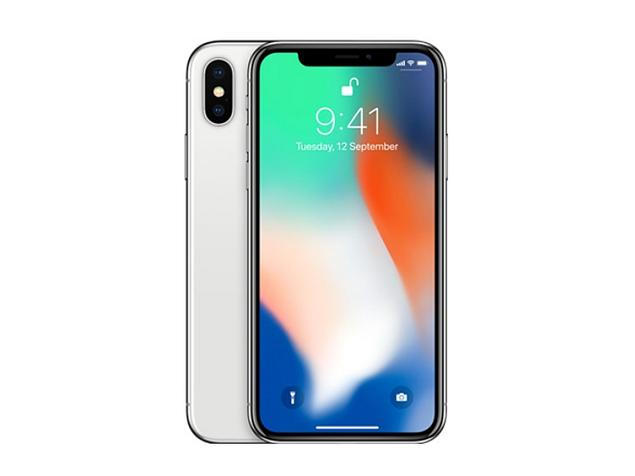
\includegraphics[width=10em,height=7em]{./images/iphone.jpg}\\
		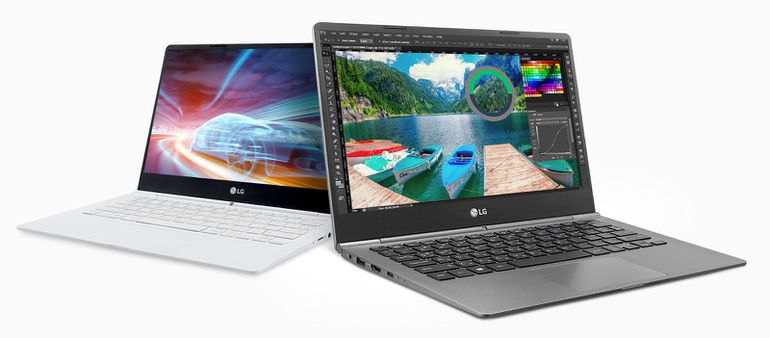
\includegraphics[width=10em,height=7em]{./images/lg-gram.jpg}\\
		\column{.3\textwidth}
		\centering
		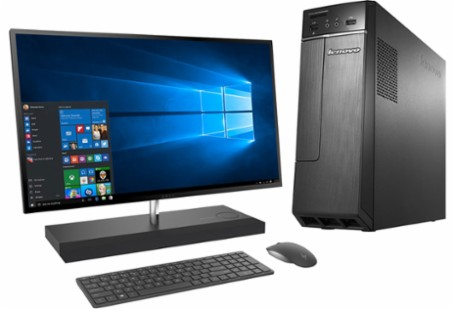
\includegraphics[width=10em,height=7em]{./images/desktop.jpg}\\
		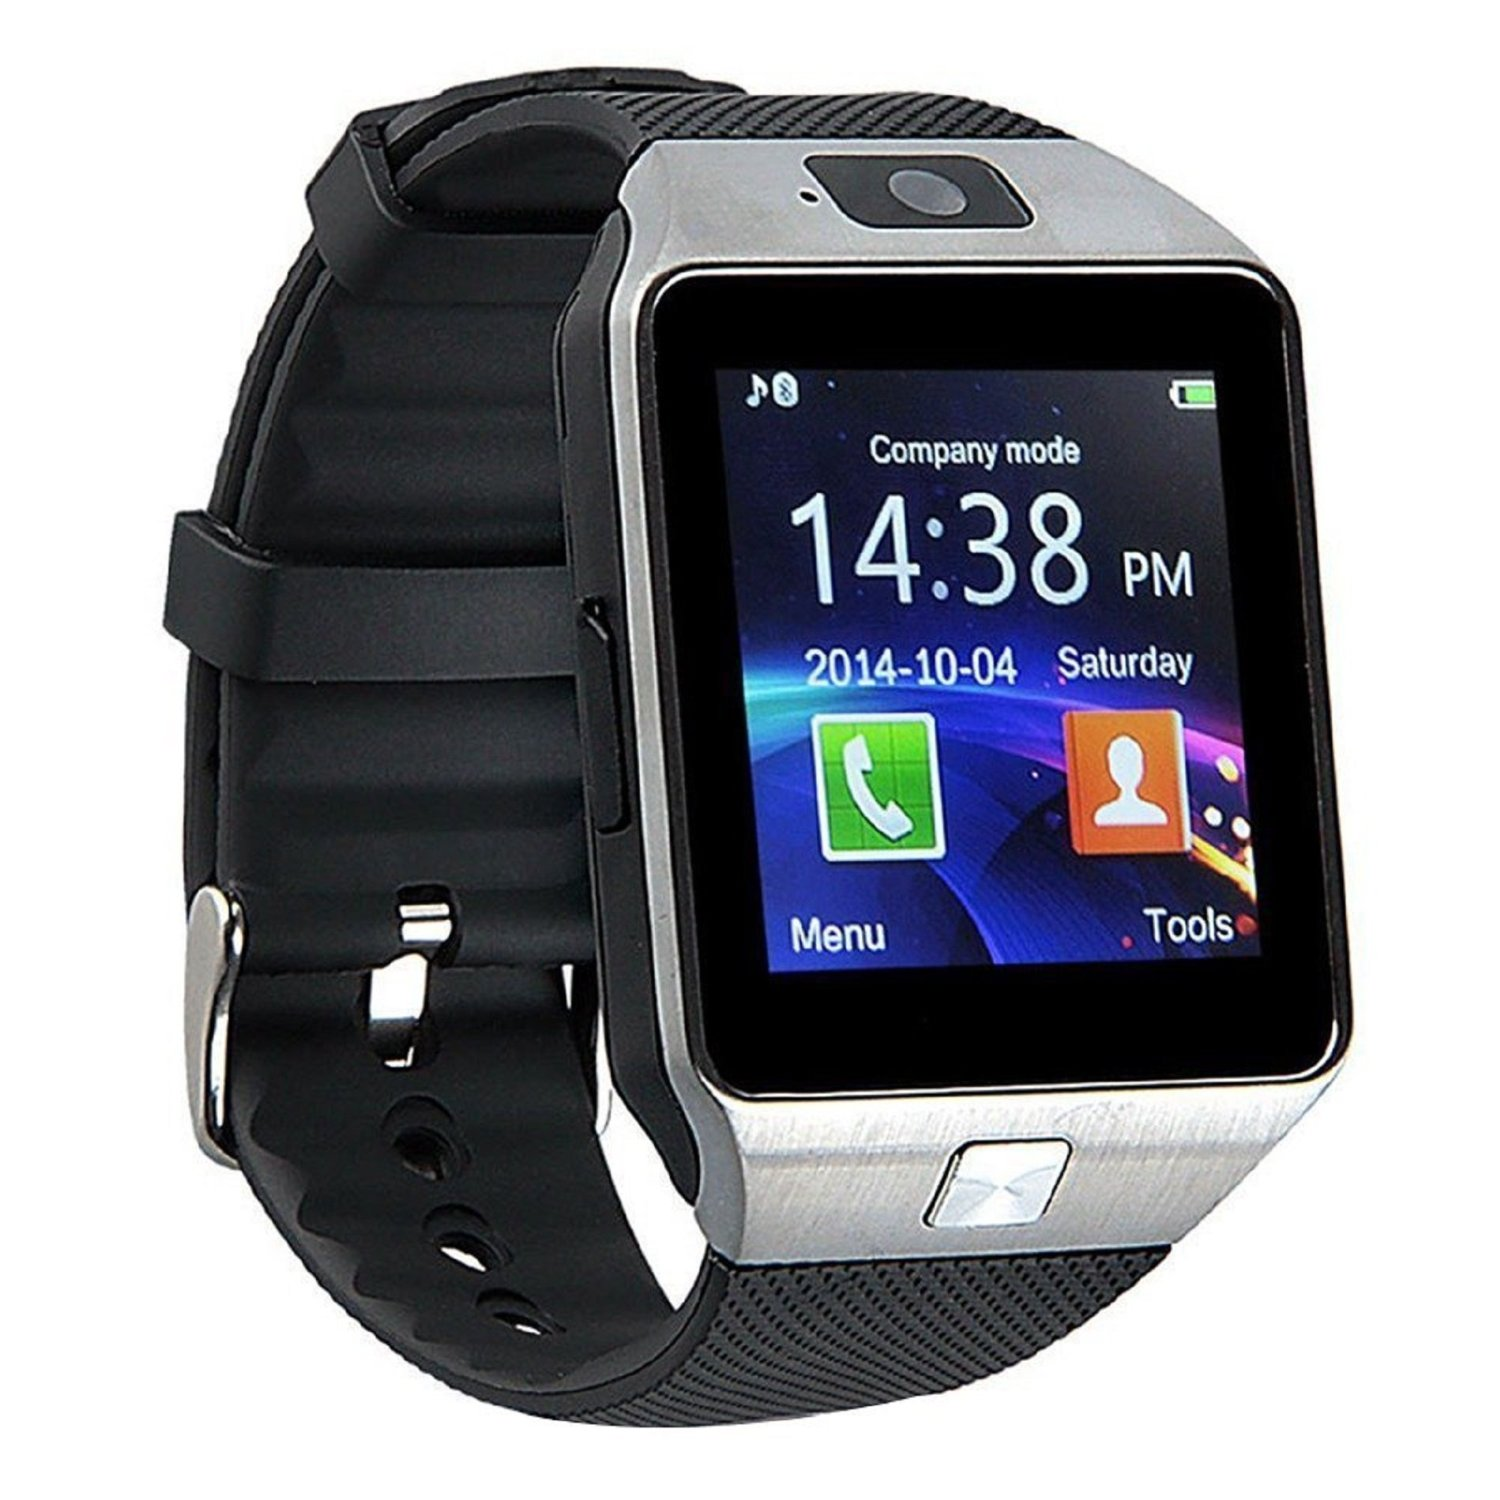
\includegraphics[width=10em,height=7em]{./images/watch.jpg}
	\end{columns}
\end{frame}

%CSL
\begin{frame}{}
  \begin{center}
    \orange{How to reason about concurrent programs?}
  \end{center}
\end{frame}


\begin{frame}{Owicki-Gries Approach}
  $$\frac{\{P_1\}~C_1~\{Q_1\}~~~\{P_2\}~C_2~\{Q_2\}}{\{P_1 \land P_2\}
    C_1~||~C_2~\{Q_1 \land Q_2\}}~~~\dagger $$
  ($\dagger$): if the proofs $\{P_1\}~C_1~\{Q_1\}$ and $\{P_2\}~C_2~\{Q_2\}$ are {\bf interference free}.
  \pause

  %% Example:
  \begin{itemize}
%%   \item Program: $\{x = 0\}~ x := x + 1 ~||~ x := x + 2 ~\{x = 3\}$
%%     \pause
%%     \item $P_1:  (x = 0 \lor x = 2)$ and $Q_1: (x = 1 \lor x = 3)$
%%     \item $P_2: (x = 0 \lor x = 1)$ and $Q_2: (x = 2 \lor x = 3)$
%%     \end{itemize}
%% \pause
%% Need to prove:
%% \begin{itemize}
%% \item $\{P_1\}~ x := x + 1~ \{Q_1\}$
%% \item $\{P_2\}~ x := x + 2 ~\{Q_2\}$
%%   \pause
\item Interference freedom: every assertion used in the local verification is
  shown not invalidated by the execution of the other processes.
%% \item $\{P_1 \land P_2\}~ x := x + 2 ~\{P_1\} $ and $\{P_2 \land P_1\} ~x := x + 1 ~\{P_2\} $
%%   \item $\{Q_1 \land P_2\}~ x := x + 2 ~\{Q_1\} $ and  $\{Q_2 \land P_1\}~ x := x + 1 ~\{Q_2\} $
\end{itemize}
\end{frame}

\begin{frame}{Owicki-Gries Approach Example}
    $$\frac{\{P_1\}~C_1~\{Q_1\}~~~\{P_2\}~C_2~\{Q_2\}}{\{P_1 \land P_2\}
    C_1~||~C_2~\{Q_1 \land Q_2\}}~~~\dagger $$
  ($\dagger$): if the proofs $\{P_1\}~C_1~\{Q_1\}$ and $\{P_2\}~C_2~\{Q_2\}$ are {\bf interference free}.

  \begin{itemize}
  \item Program: $\{x = 0\}~ x := x + 1 ~||~ x := x + 2 ~\{x = 3\}$
  %% \item $P_1:  (x = 0 \lor x = 2)$ and $Q_1: (x = 1 \lor x = 3)$
  %% \item $P_2: (x = 0 \lor x = 1)$ and $Q_2: (x = 2 \lor x = 3)$
  \item $P_1:  (x = 0 \lor x = 2)$ and $Q_1: (x = 1 \lor x = 3)$
  \item $P_2: (x = 0 \lor x = 1)$ and $Q_2: (x = 2 \lor x = 3)$
  \end{itemize}
\pause
Need to prove:
\begin{itemize}
\item $\{P_1\}~ x := x + 1~ \{Q_1\}$
\item $\{P_2\}~ x := x + 2 ~\{Q_2\}$
  \pause
  \item $\{P_1 \land P_2\}~ x := x + 2 ~\{P_1\} $ and $\{P_2 \land P_1\} ~x := x + 1 ~\{P_2\} $
  \item $\{Q_1 \land P_2\}~ x := x + 2 ~\{Q_1\} $ and  $\{Q_2 \land P_1\}~ x := x + 1 ~\{Q_2\} $
  %%   \pause
  %% \item   $\{(x = 0 \lor x = 2) \land (x = 0 \lor x = 1)\}~x := x + 2~\{x = 0 \lor x = 2\}$
  %% \item   $\{(x = 1 \lor x = 3) \land (x = 0 \lor x = 1)\}~x := x + 2~\{x = 1 \lor x = 3\}$
  %% \item   $\{(x = 0 \lor x = 1) \land (x = 0 \lor x = 2)\}~x := x + 1~\{x = 0 \lor x = 1\}$
  %% \item   $\{(x = 2 \lor x = 3) \land (x = 0 \lor x = 2)\}~x := x + 1~\{x = 2 \lor x = 3\}$
\end{itemize}

\end{frame}

%Rely Guarantee
\begin{frame}{Rely Guarantee Reasoning (P,R,G,Q)}
  \begin{itemize}
  \item Precondition P and Postcondition Q.
  \item The rely condition R models all the atomic actions of the environment,
    describing the interference the  program can tolerate from its environment.
  \item The guarantee condition G models the atomic actions of the program, and
    hence decribing the interference that it imposes on the other threads of the system.
  \end{itemize}
  \pause
  $$\frac{C_1 \models (p_1, R_1,G_1,q_1)~~~~~~ C_2 \models (p_2, R_2, G_2, q_2)}{C_1~||~C_2 \models (p_1 \land
    p_2, R_1 \land R_2, G_1 \lor G_2, q_1 \land q_2)} \dagger$$

  ($\dagger$): The precondition $P_i$ is \text{stable} under rely condition $R_i$.
\end{frame}

\begin{frame}{Rely Guarantee Example}
     $$\frac{C_1 \models (p_1, R_1,G_1,q_1)~~~~~~ C_2 \models (p_2, R_2, G_2,
    q_2)}{C_1~||~C_2 \models (p_1 \land 
    p_2, R_1 \land R_2, G_1 \lor G_2, q_1 \land q_2)}$$
 
  Program: $\{x = 0\}~ x := x + 1 ~||~ x := x + 2 ~\{x = 3\}$ \\
  New form: $x := x + 1 ~||~ x := x + 2~~\models (x=0, x' = x, True, x' = 3)$
  with \textbf{True} denotes the action that changes the state arbitrarily. 
    \pause
  \begin{equation}
    \begin{split}
      x := x + 1 ~\models &~(x = 0 \lor x = 2, \\
      &(x = 0 \land x' = 2) \lor (x = 1 \land x' = 3), \\
      &(x = 0 \land x'=1) \lor (x=2 \land x' = 3), \\
      &(x = 0 \land x' = 1) \lor (x = 2 \land x' = 3)) \nonumber
  \end{split}
  \end{equation}
  \pause
  \begin{equation}
    \begin{split}
      x := x + 2 ~\models &~(x = 0 \lor x = 1, \\
      &(x = 0 \land x' = 1) \lor (x = 2 \land x' = 3), \\
      &(x = 0 \land x'= 2) \lor (x=1 \land x' = 3), \\
      &(x = 0 \land x' = 2) \lor (x = 1 \land x' = 3)) \nonumber
  \end{split}
  \end{equation}
\end{frame}

%% Remark: R and G are quite complicated, how marriage of RG and CSL resolve it?
%% Dont' scare to make a question

\begin{frame}{Concurrent Separation Logic - CSL}
  \begin{itemize}
  \item Interference-free concurrency
    $$\frac{\{P_1\}~C_1~\{Q_1\}~~~\{P_2\}~C_2~\{Q_2\}}{\{P_1 \ast P_2\}~C_1~||~C_2 ~\{Q_1 \ast Q_2
    \}}$$
    \pause
  \item A resource invariant $RI_r$ is associated with each resource. Acquiring
    the resource imports the resource invariant in the local scope.
    $$\frac{\{(P \ast RI_r) \land S\}~C~\{Q \ast RI_r\}}{\{P\}~with~r~when~S~do~C~\{Q\}}$$
  \end{itemize}
\end{frame}

\begin{frame}{CSL tree}
  \begin{figure}
  	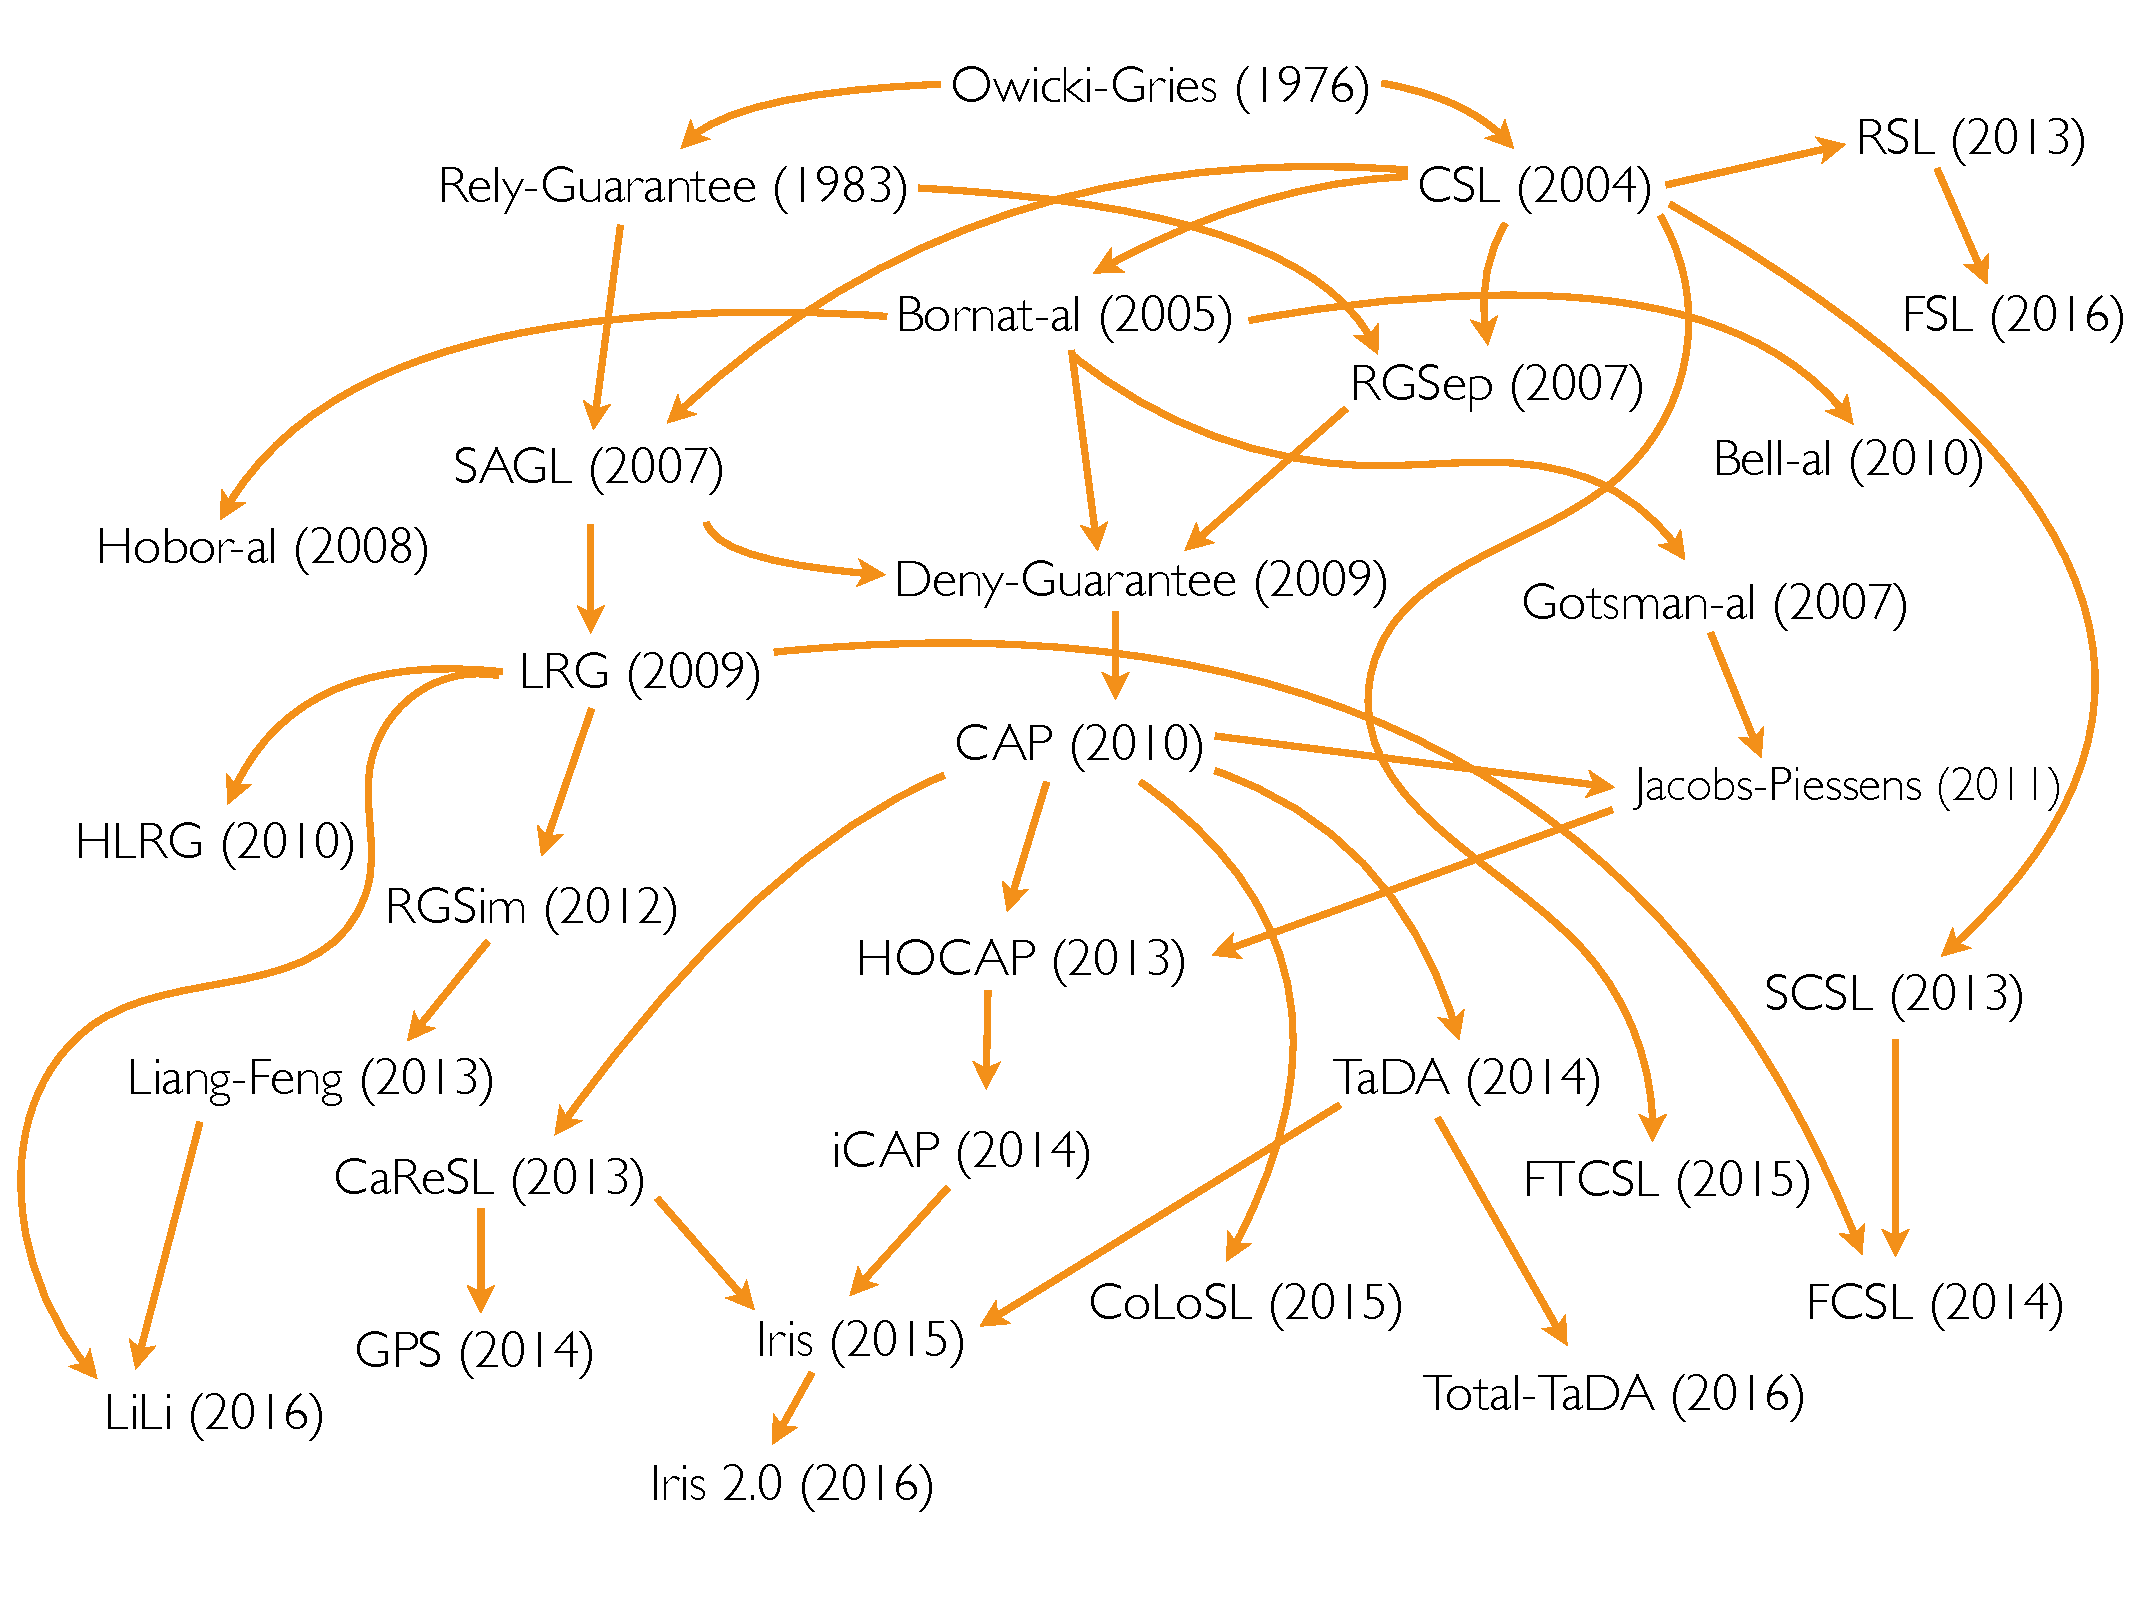
\includegraphics[width=26em,height=20em]{./images/CSL-Family-Tree.pdf}
  \end{figure}
\end{frame}
  %% \begin{frame}{How to reason about concurrent programs?}
%%   \begin{itemize}

%%   \item A new breakthough: Concurrent separation logic
%%   \item Built on the success of Sequential Separation Logic
%%   \item Godel Award 2016

%%   \end{itemize}
%% \end{frame}
% First example
\begin{frame}{Automated tools for CSL?}
  \begin{itemize}
  \item Great successes of sequential separation logic tools, e.g. Infer of
    Facebook, and SLAyer of Microsoft. 
  \item Only 2 CSL tools appear \textit{this year}, Caper and Starling.
    \pause
  \item Our contributions:
    \begin{itemize}
    \item The first formal verification for {\CDL} by using abstract predicates.
    %% \item A modular solution to the counter mechanism by combining a
    %%   \textit{thread-local} abstraction and the \textit{global} view.
    \item Ensure race-freedom and deadlock-freedom.
    \item An automated prototype which can verify a library implemenation of {\CDL}.
    \end{itemize}
  \end{itemize}
 \end{frame}

\begin{frame}{Motivation Example}
\begin{figure}

\centering
\code{c = \createlatch(2);}

\vspace{-12pt}
\[
\left(
\begin{tabular}{ 
  l@{\extracolsep{\fill}} || 
  l@{\extracolsep{\fill}} || 
  l@{\extracolsep{\fill}} }
\BCOMMENT{\SPEC{$T_1$}} & \BCOMMENT{\SPEC{$T_2$}} & \BCOMMENT{\SPEC{$T_3$}}\\
\code{h=hs*cosine($\theta$/2);} & 
\code{r=hs*sine($\theta$/2);} & \\
\code{countDown(c);} & \code{countDown(c);} & \code{await(c);}\\
& & \code{V=(1/3)*$\pi$*power(r,2)*h;}\\
\end{tabular}\!\!\right)%\!\!\code{;}
\]

\begin{tabular}{ll}
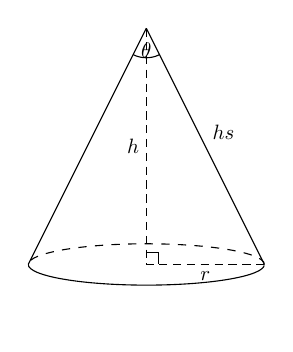
\begin{tikzpicture}[scale=0.75, every node/.style={transform shape}]
 \begin{scope}
   \clip (-2,0) rectangle (2,1cm);
   \draw[dashed] (0,0) circle (2cm and 0.35cm);
 \end{scope}
 \begin{scope}
   \clip (-2,0) rectangle (2,-1cm);
   \draw (0,0) circle (2cm and 0.35cm);
 \end{scope}
   \draw[densely dashed]
        (0,4) coordinate (c)
     -- node[auto=right] {$h$}            %,font=\footnotesize
        coordinate[pos=0.95] (aa) (0,0)
     -- node[below] {$r$} 
        coordinate[pos=0.1]  (bb) (2,0);
   \draw (aa) -| (bb);
   \draw (c) -- (-2,0) coordinate (a);
   \draw (c) -- node [auto=left] {$hs$} 
                (2,0) coordinate (b);
   \begin{scope}
     \path[clip] (a) -- (c) -- (b) -- cycle;
     \draw (c) circle (5mm) node [label=below:$\theta$]{};
   \end{scope}    
\end{tikzpicture}

&
\pause
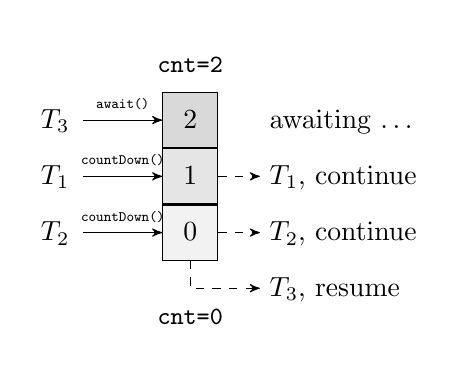
\begin{tikzpicture}[every node/.style={anchor=base,
    text height=.8em,text depth=.2em,minimum size=7mm},
    ->, >=stealth']
    
  \matrix{
    \node[] (lbl) {\code{cnt=2}};\\
    %\node[fill=gray!30] (cnt_init) {$2$};\\
    \node[fill=gray!30,draw] (cnt_2) {$2$};\\
    \node[fill=gray!20,draw] (cnt_1) {$1$};\\
    \node[fill=gray!10,draw] (cnt_0) {$0$};\\
    \node[] (cnt_end) {};\\
  };
  
    \node[left= of cnt_2] (tm) {$T_3$};
    \node[left= of cnt_1] (t1) {$T_1$};
    \node[left= of cnt_0] (t2) {$T_2$};
  
    \node[right=15pt of cnt_2] (wait) {awaiting $\ldots$};
    \node[right=15pt of cnt_1] (cont_1) {$T_1$, continue};
    \node[right=15pt of cnt_0] (cont_2) {$T_2$, continue};
    \node[right=15pt of cnt_end] (cont_m) {$T_3$, resume};
  
  \path (tm) edge node [->, scale=.58, auto] {\code{await()}} (cnt_2);
  \path (t1) edge node [->, scale=.58, auto] {\code{countDown()}} (cnt_1);
  \path (t2) edge node [->, scale=.58, auto] {\code{countDown()}} (cnt_0);
  
  %\draw [->, dashed] (cnt_2) to node [] {} (wait);
  \draw [->, dashed] (cnt_1) -- node [] {} (cont_1);
  \draw [->, dashed] (cnt_0) -- node [] {} (cont_2);
  \draw [->, dashed, auto] (cnt_0) |- node [below] {\code{cnt=0}} (cont_m);
\end{tikzpicture}
\end{tabular}

\end{figure}

\end{frame}

% Second example
\begin{frame}{Motivation Example}
  \begin{itemize}
    \item Resources can be split and sent to multiple receiving threads.
    \end{itemize}
\begin{center}
\code{c = \createlatch(1);}
\[
{
\left(
\begin{tabular}{ l@{\extracolsep{\fill}} || 
                 l@{\extracolsep{\fill}} || 
                 l@{\extracolsep{\fill}} }
\BCOMMENT{\SPEC{send P*Q}} ~&~ \code{await(c);} ~&~ \code{await(c);}\\
\code{countDown(c);} ~&~ \BCOMMENT{\SPEC{receive P}} ~&~ \BCOMMENT{\SPEC{receive Q}}\\
\code{\ldots} ~&~ \code{\ldots} ~&~ \code{\ldots}\\
\end{tabular}\right)
}
\]
\end{center}

\end{frame}
%example
\begin{frame}{Motivation Example}
  \begin{itemize}
    \item Model the barrier synchronization.
    \end{itemize}
\begin{center}
\code{c = \createlatch(2);}
\[
{
\left(
\begin{tabular}{ l@{\extracolsep{\fill}}  || l@{\extracolsep{\fill}} }
\code{\ldots} ~&~\code{\ldots}\\
\BCOMMENT{\SPEC{owns P}} ~&~ \BCOMMENT{\SPEC{owns Q}}\\
\code{countDown(c);~await(c);} ~&~\code{countDown(c);~await(c);}\\
\BCOMMENT{\SPEC{owns Q}} ~&~ \BCOMMENT{\SPEC{owns P}}\\
\code{\ldots} ~&~\code{\ldots}\\
\end{tabular}\right)
}
\]
\end{center}
\end{frame}

%concurrent abstract predicates for CDL
\begin{frame}{Resource Predicates}
\[
\begin{array}{l}
\code{\CDL~\createlatch(n)~with~P}\\
\SPEC{~~~~\requires~\code{n\sm{\gt}0}} \\
\SPEC{~~~~\ensures~ \LatchIn{res}{P} {\sep}\LatchOut{res}{P}{\sep}\code{CNT(res,n)}}; \\
\SPEC{~~~~\requires~\code{n\sm{=}0}} \\
\SPEC{~~~~\ensures~ \code{CNT(res,-1)}}; \\
\end{array}
\]
\end{frame}

\begin{frame}{Resource Predicates}
\[
\begin{array}{l}
\code{void~countDown(\CDL~i)}\\
~~
\SPEC{\requires~\LatchIn{i}{P}{\sep}\code{P}{\sep}\code{CNT(i,n)}\sm{\wedge}\code{n{>}0}}\\ 
~~ \SPEC{\ensures~ \code{CNT(i,n{-}1)}};\\ 
~~
\SPEC{\requires~\code{CNT(i,-1)}}\\
~~ \SPEC{\ensures~ \code{CNT(i,-1)}};\\
\\
\\
\pause
\code{void~await(\CDL~i)}\\
~~ \SPEC{\requires~\LatchOut{i}{P}{\sep}\code{CNT(i,0)}}\\
~~ \SPEC{\ensures~ \code{P}{\sep}\code{CNT(i,-1)}};\\
~~ \SPEC{\requires~\code{CNT(i,-1)}}\\
~~ \SPEC{\ensures~ \code{CNT(i,-1)}};%\\
\end{array}
\]
\end{frame}

\begin{frame}[shrink=17]{Splitting Lemmas}
%% \begin{center}
%% \begin{small}
%% \[
%% \begin{array}{l}
%% \BSPEC{\normrulen{1}:

%% \CNT{c}{n} {\sep} \CNT{c}{-1} {\wedge} \code{n\sm{\leq}0} {\longrightarrow} \CNT{c}{-1}}
%% \\
%% \BSPEC{\normrulen{2}:
%% \CNT{c}{n1} {\sep} \CNT{c}{n2}\, {\wedge}\, \code{n}{=}\code{n1{+}n2} \,{\wedge}\, \code{n1,n2}{\geq}\code{0} 
%% {\longrightarrow} \CNT{c}{n}}
%% \\
%% \BSPEC{\normrulen{3}:
%% \LatchOut{c}{P} {\sep} \CNT{c}{-1}  {\longrightarrow} \CNT{c}{-1}{\sep}\code{P}}
%% \end{array}
%% \]
%% \end{small}
%% \end{center}
%% \pause
%%%%%%%%%%%%%%%%%%% Other rules
\begin{small}
\[
\begin{array}{l}
\BSPEC{\splitrulen{1}:
\LatchOut{i}{P{\sep}Q} \,{\longrightarrow}\, \LatchOut{i}{P} {\sep}\LatchOut{i}{Q}}
\\
\BSPEC{\splitrulen{2}:
\LatchIn{i}{P{\sep}Q} \,{\longrightarrow}\, \LatchIn{i}{P} {\sep}\LatchIn{i}{Q}}
\\
\BSPEC{\splitrulen{3}:
\CNT{c}{n} \,{\wedge}\, %% \code{n1}{\geq}\code{{-}1}  \,{\wedge}\,
\code{n1,n2}{\geq}\code{0}  \, {\wedge}\, \code{n}{=}\code{n1{+}n2} 
\,{\longrightarrow}\,
\CNT{c}{n1} {\sep} \CNT{c}{n2} }
\end{array}
\]
\end{small}

\pause
\begin{center}
\begin{small}
\code{c = \createlatch(2)~with~\SPEC{P{\sep}Q};} \\
\code{\CSPEC{\LatchOut{c}{P{\sep}Q}{\sep}\LatchIn{c}{P{\sep}Q}{\sep}\CNT{c}{2}}} \\
\code{\CSPEC{\LatchOut{c}{P{\sep}Q}{\sep}\LatchIn{c}{P}{\sep}\LatchIn{c}{Q}{\sep}\CNT{c}{0}{\sep}\CNT{c}{1}{\sep}\CNT{c}{1}}} \\\vspace{-12pt}
\[
\left(
\begin{tabular}{ 
  l@{\extracolsep{\fill}} || 
  l@{\extracolsep{\fill}} || 
  l@{\extracolsep{\fill}} }
%% \code{\saying{$T_m$}} & \code{\saying{$T_1$}} & \code{\saying{$T_2$}}\\
\code{\dotonly{}} & \code{\dotsaying{create P}} & \code{\dotsaying{create Q}}\\
\!\!\code{\CSPEC{\!\!\LatchOut{c}{P{\sep}Q}{\sep}\CNT{c}{0}}}
& \code{\CSPEC{\!\!P{\sep}\LatchIn{c}{P}{\sep}\CNT{c}{1}}} 
& \code{\CSPEC{\!\!Q{\sep}\LatchIn{c}{Q}{\sep}\CNT{c}{1}}} \\
\!\!\code{await(c);} & \code{countDown(c);} & \code{countDown(c);}\\
\!\!\code{\CSPEC{{P{\sep}Q{\sep}\CNT{c}{-1}}}}
& \code{\CSPEC{\CNT{c}{0}}} 
& \code{\CSPEC{\CNT{c}{0}}} \\
\code{\dotsaying{use P*Q}} & \code{\dotonly{}} & \code{\dotonly{}} \\
%% \code{\ldots} & & \\
\end{tabular}\!\!\right)%\!\!\code{;}
\]
\end{small}
\end{center}

\end{frame}

% Race error
\begin{frame}{Race Condition}
\begin{center}
  \begin{small}
\code{c = \createlatch(1)~with~\SPEC{P{\sep}Q};} 
\\\vspace{-12pt}
\[
\left(
\begin{tabular}{ 
  l@{\extracolsep{\fill}} || 
  l@{\extracolsep{\fill}} || 
  l@{\extracolsep{\fill}} }
\code{\dotonly{}} & \code{\dotsaying{create P}} & \code{\dotsaying{create Q}} \\
%% \!\!\code{\CSPEC{\!\!\LatchOut{c}{P{\sep}Q}{\sep}\CNT{c}{0}}}
%% &\code{\CSPEC{\!\!P{\sep}\LatchIn{c}{P}{\sep}\CNT{c}{1}}} 
%% & \code{\CSPEC{\!\!Q{\sep}\LatchIn{c}{Q}{\sep}\CNT{c}{0}}} \\
\code{await(c);} & \code{countDown(c);} & \code{skip();}\\
%% \!\!\code{\CSPEC{\!\!{P{\sep}Q{\sep}\CNT{c}{-1}}}}
%% & \code{\CSPEC{\!\!\CNT{c}{0}}} 
%% & \code{\CSPEC{\!\!Q{\sep}\LatchIn{c}{Q}{\sep}\CNT{c}{0}}} \\
\code{\dotsaying{use P*Q}} & \code{\dotonly{}} & \code{\dotonly{}} \\
\end{tabular}\!\!\right)%\!\!\code{;}
\]

\end{small}
\end{center}

\begin{itemize}
\item The first thread uses \code{Q} while it's not ready for use.
\end{itemize}
\end{frame}


\begin{frame}[shrink=17]{Race Error}
  \BSPEC{\errrulen{1}:
    \LatchIn{c}{P}{\sep}\code{CNT(c,-1)}
    \sm{\longrightarrow} \RACE}  
\pause
    %% \begin{figure}
\begin{center}
  \begin{small}
\code{c = \createlatch(1)~with~\SPEC{P{\sep}Q};} \\
\code{\CSPEC{\LatchOut{c}{P{\sep}Q}{\sep}\LatchIn{c}{P{\sep}Q}{\sep}\CNT{c}{1}}} \\
\code{\CSPEC{\LatchOut{c}{P{\sep}Q}{\sep}\LatchIn{c}{P}{\sep}\LatchIn{c}{Q}{\sep}\CNT{c}{0}{\sep}\CNT{c}{1}{\sep}\CNT{c}{0}}}
\\\vspace{-12pt}
\[
\left(
\begin{tabular}{ 
  l@{\extracolsep{\fill}} || 
  l@{\extracolsep{\fill}} || 
  l@{\extracolsep{\fill}} }
\code{\dotonly{}} & \code{\dotsaying{create P}} & \code{\dotsaying{create Q}} \\
\!\!\code{\CSPEC{\!\!\LatchOut{c}{P{\sep}Q}{\sep}\CNT{c}{0}}}
&\code{\CSPEC{\!\!P{\sep}\LatchIn{c}{P}{\sep}\CNT{c}{1}}} 
& \code{\CSPEC{\!\!Q{\sep}\LatchIn{c}{Q}{\sep}\CNT{c}{0}}} \\
\code{await(c);} & \code{countDown(c);} & \code{skip();}\\
\!\!\code{\CSPEC{\!\!{P{\sep}Q{\sep}\CNT{c}{-1}}}}
& \code{\CSPEC{\!\!\CNT{c}{0}}} 
& \code{\CSPEC{\!\!Q{\sep}\LatchIn{c}{Q}{\sep}\CNT{c}{0}}} \\
\code{\dotsaying{use P*Q}} & \code{\dotonly{}} & \code{\dotonly{}} \\
\end{tabular}\!\!\right)%\!\!\code{;}
\]

\code{\CSPEC{{P{\sep}Q{\sep}\CNT{c}{-1}}
 \sep \CNT{c}{0} 
 \sep Q{\sep}\LatchIn{c}{Q}{\sep}\CNT{c}{0}}} \\
\code{\CSPEC{{P{\sep}Q{\sep}\CNT{c}{-1}}
 \sep Q{\sep}\LatchIn{c}{Q}}} \\
\code{\CSPEC{{\color{red} RACE-ERROR detected
by \errrulen{1} }}} 

\end{small}
\end{center}
%% \caption{A {\CDL} with a race error}\label{figure.cdl.1}
%% \end{figure}

\end{frame}

\begin{frame}[shrink=17]{Race Error}
  
%% \begin{figure}
\begin{center}
  \begin{small}
\code{c = \createlatch(1)~with~\SPEC{P{\sep}Q};} \\
\code{\CSPEC{\LatchOut{c}{P{\sep}Q}{\sep}\LatchIn{c}{P{\sep}Q}{\sep}\CNT{c}{1}}} \\
\code{\CSPEC{\LatchOut{c}{P{\sep}Q}{\sep}\LatchIn{c}{P}{\sep}\LatchIn{c}{Q}{\sep}\CNT{c}{0}{\sep}\CNT{c}{1}{\sep}\CNT{c}{0}}}
\\\vspace{-12pt}
\[
\left(
\begin{tabular}{ 
  l@{\extracolsep{\fill}} || 
  l@{\extracolsep{\fill}} || 
  l@{\extracolsep{\fill}} }
\code{\dotonly{}} & \code{\dotsaying{create P}} & \code{\dotsaying{create Q}} \\
\!\!\code{\CSPEC{\!\!\LatchOut{c}{P{\sep}Q}{\sep}\CNT{c}{0}}}
&\code{\CSPEC{\!\!P{\sep}\LatchIn{c}{P}{\sep}\CNT{c}{1}}} 
& \code{\CSPEC{\!\!Q{\sep}\LatchIn{c}{Q}{\sep}\CNT{c}{0}}} \\
\code{await(c);} & \code{countDown(c);} & \code{countDown(c);}\\
\!\!\code{\CSPEC{\!\!{P{\sep}Q{\sep}\CNT{c}{-1}}}}
& \code{\CSPEC{\!\!\CNT{c}{0}}} 
& \code{\CSPEC{\color{red} RACE-ERROR}} \\
%% \code{\dotsaying{use P*Q}} & \code{\dotonly{}} & \code{\dotonly{}} \\
\end{tabular}\!\!\right)%\!\!\code{;}
\]
%%  \sep \CNT{c}{0} 
%%  \sep Q{\sep}\LatchIn{c}{Q}{\sep}\CNT{c}{0}}} \\
%% \code{\CSPEC{{P{\sep}Q{\sep}\CNT{c}{-1}}
%%  \sep Q{\sep}\LatchIn{c}{Q}}} \\
%% \code{\CSPEC{{\color{red} RACE-ERROR detected
%% by \errrulen{1} }}} 

\end{small}
\end{center}

  \begin{itemize}
    \item The precondition of {\CD} cannot be \code{CNT(c,0)}
  \end{itemize}
\end{frame}

\begin{frame}[shrink=17]{Race Error}
  
%% \begin{figure}
\begin{center}
  \begin{small}
\code{c = \createlatch(2)~with~\SPEC{P{\sep}Q};} \\
\code{\CSPEC{\LatchOut{c}{P{\sep}Q}{\sep}\LatchIn{c}{P{\sep}Q}{\sep}\CNT{c}{2}}} \\
\code{\CSPEC{\LatchOut{c}{P{\sep}Q}{\sep}\LatchIn{c}{P}{\sep}\LatchIn{c}{Q}{\sep}\CNT{c}{0}{\sep}\CNT{c}{1}{\sep}\CNT{c}{1}}}
\\\vspace{-12pt}
\[
\left(
\begin{tabular}{ 
  l@{\extracolsep{\fill}} || 
  l@{\extracolsep{\fill}} || 
  l@{\extracolsep{\fill}} }
\code{\dotonly{}} & \code{\dotsaying{create P}} & \code{\dotsaying{create Q}} \\
\!\!\code{\CSPEC{\!\!\LatchOut{c}{P{\sep}Q}{\sep}\CNT{c}{0}}}
&\code{\CSPEC{\!\!P{\sep}\LatchIn{c}{P}{\sep}\CNT{c}{1}}} 
& \code{\CSPEC{\!\!Q{\sep}\LatchIn{c}{Q}{\sep}\CNT{c}{1}}} \\
\code{await(c);} & \code{countDown(c);} & \code{countDown(c);}\\
\!\!\code{\CSPEC{\!\!{P{\sep}Q{\sep}\CNT{c}{-1}}}}
& \code{\CSPEC{\!\!\CNT{c}{0}}} 
& \code{\CSPEC{\!\!\CNT{c}{0}}} \\
\code{\dotsaying{use P*Q}} & \code{\dotonly{}} & \code{\dotonly{}} \\
\end{tabular}\!\!\right)%\!\!\code{;}
\]

\code{\CSPEC{{P{\sep}Q{\sep}\CNT{c}{-1}}
 \sep \CNT{c}{0} 
 \sep \CNT{c}{0}}} \\
\code{\CSPEC{{P{\sep}Q{\sep}\CNT{c}{-1}}
 \sep \CNT{c}{0}}} \\
\code{\CSPEC{{P{\sep}Q{\sep}\CNT{c}{-1}}
}} \\

\end{small}
\end{center}

\pause
  \begin{center}
\begin{small}
\[
\begin{array}{l}
\BSPEC{\normrulen{1}:

\CNT{c}{n} {\sep} \CNT{c}{-1} {\wedge} \code{n\sm{\leq}0} {\longrightarrow} \CNT{c}{-1}}
\\
\BSPEC{\normrulen{2}:
\CNT{c}{n1} {\sep} \CNT{c}{n2}\, {\wedge}\, \code{n}{=}\code{n1{+}n2} \,{\wedge}\, \code{n1,n2}{\geq}\code{0} 
{\longrightarrow} \CNT{c}{n}}
%% \\
%% \BSPEC{\normrulen{3}:
%% \LatchOut{c}{P} {\sep} \CNT{c}{-1}  {\longrightarrow} \CNT{c}{-1}{\sep}\code{P}}
\end{array}
\]
\end{small}
\end{center}

\end{frame}

% Deadlock
\begin{frame}{Deadlock}
%%   \BSPEC{\errrulen{2}: 
%% \code{CNT(c,a)}{\sep}\code{CNT(c,-1)}\sm{\wedge}\code{a{>}0} 
%% \sm{\longrightarrow} \DEADLOCK}
%% \pause
\begin{center}
\begin{small}
\code{c = \createlatch(2);}
%% \code{\CSPEC{CNT(c,2) {\LRA} CNT(c,2){\sep}CNT(c,0)}}\\
\[
{
\left(
\begin{tabular}{ l@{\extracolsep{\fill}}  || l@{\extracolsep{\fill}} }
%% \code{\CSPEC{CNT(c,2)}} &~~\code{\CSPEC{CNT(c,0)}}\\
\code{countDown(c);~~} &~~\code{await(c);}\\
%% \code{\CSPEC{CNT(c,1)}} &~~\code{\CSPEC{CNT(c,-1)}}\\
\end{tabular}\right)\code{;}
}
\]

%% \code{\CSPEC{CNT(c,1){\sep}CNT(c,-1)}}% \sm{\longrightarrow} \DEADLOCK}}
%% \\
%% \code{\CSPEC{{\color{red}{\DEADLOCK} detected by \errrulen{2}}}}
\end{small}
\end{center}
%% \end{frame}
\pause
%% \begin{frame}{Deadlock}
  \BSPEC{\errrulen{2}: 
\code{CNT(c,a)}{\sep}\code{CNT(c,-1)}\sm{\wedge}\code{a{>}0} 
\sm{\longrightarrow} \DEADLOCK}
\pause
\begin{center}
\begin{small}
\code{c = \createlatch(2);}
\\
\code{\CSPEC{CNT(c,2) {\LRA} CNT(c,2){\sep}CNT(c,0)}}\\
\[
{
\left(
\begin{tabular}{ l@{\extracolsep{\fill}}  || l@{\extracolsep{\fill}} }
\code{\CSPEC{CNT(c,2)}} &~~\code{\CSPEC{CNT(c,0)}}\\
\code{countDown(c);~~} &~~\code{await(c);}\\
\code{\CSPEC{CNT(c,1)}} &~~\code{\CSPEC{CNT(c,-1)}}\\
\end{tabular}\right)\code{;}
}
\]

\code{\CSPEC{CNT(c,1){\sep}CNT(c,-1)}}% \sm{\longrightarrow} \DEADLOCK}}
\\
\code{\CSPEC{{\color{red}{\DEADLOCK} detected by \errrulen{2}}}}
\end{small}
\end{center}
\end{frame}
%%%%%%%%%%%%%%%%%%%%%%%%%%%%%%%%%%%%%%%%%%
\begin{frame}{Inter-latch Deadlock}
  \begin{small}
\begin{center}
\code{c1 = \createlatch(1); c2 = \createlatch(1);}\\
%% \CSPEC{WAIT\{\} $\ast$ CNT(c1,1) $\ast$ CNT(c2,1)
%%   $\Longrightarrow$ }  \\
%% \CSPEC{CNT(c1,1) {\sep} CNT(c2,0) {\sep} CNT(c2,1) {\sep} CNT(c1,0) }\\
\[
{
\left(
\begin{tabular}{ l@{\extracolsep{\fill}}  || l@{\extracolsep{\fill}} }
%% \CSPEC{CNT(c1,1){\sep}CNT(c2,0)} &~~\CSPEC{CNT(c2,1){\sep}CNT(c1,0)}\\
\code{await(c2);~~} &~~\code{await(c1);}\\
%% \CSPEC{CNT(c1,1){\sep}CNT(c2,-1)} &~~\CSPEC{CNT(c2,1){\sep}CNT(c1,-1)}\\
%% \CSPEC{$\ast$ WAIT(\{c2 $\rightarrow$ c1\})} &~~ \CSPEC{$\ast$ WAIT(\{c1 $\rightarrow$ c2\})}\\
\code{countDown(c1);~~} &~~\code{countDown(c2);}\\
%% \CSPEC{CNT(c1,0){\sep}CNT(c2,-1)} &~~\CSPEC{CNT(c2,0){\sep}CNT(c1,-1)}\\
%% \CSPEC{$\ast$ WAIT(\{c2 $\rightarrow$ c1\})} &~~ \CSPEC{$\ast$ WAIT(\{c1 $\rightarrow$ c2\})}\\
\end{tabular}\right)%\code{;}
}
\]

%% \CSPEC{\quad CNT(c1,-1){\sep}CNT(c2,-1) {\sep} WAIT(\{c2 $\rightarrow$ c1, c1
%%   $\rightarrow$ c2\})} \\ 
%% \code{\CSPEC{{\color{red}{\DEADLOCK} detected by \errrulen{3} }}}

\end{center}
\end{small}
\pause
  \BSPEC{\waitrulen{1}:
  \WAITC{\code{S}}\sm{{\wedge}\neg}\code{isCyclic(S)}\sm{\longrightarrow}
  \WAITC{\{\}} } \\
  \BSPEC{\waitrulen{2}: 
  \code{CNT($c_1$,a)} {\sep}\code{CNT($c_2$,-1)} {\sep} \WAITC{\code{S}} $\land$
  \code{a{>}0} $\longrightarrow$ } \\
  \BSPEC{\text{\ \ \ \ \ \ \ \ \ \ \ \ \ }\code{CNT($c_1$,a)}{\sep}\code{CNT($c_2$,-1)}\sm{\wedge}\code{a{>}0}
    {\sep} \WAITC{\code{S}{\cup}\code{\{$c_2${\ra}$c_1$\}}}}\\
  \BSPEC{\waitrulen{3}: \WAITC{\code{$S_1$}} {\sep} \WAITC{\code{$S_2$}}
    \sm{\longleftrightarrow} \WAITC{(\code{$S_1 \cup S_2$}) } } \\
  \BSPEC{\errrulen{3}: \WAITC{\code{S}} \code{\sm{\wedge}~isCyclic(S)} \sm{\longrightarrow} \DEADLOCK }

\end{frame}

\begin{frame}{Inter-latch Deadlock}
  %% \begin{center}
  %%   \code{c1 = \createlatch(1); c2 = \createlatch(1);}
  %%   \code{\CSPEC{\addperm{\WAIT{}}{1}{\sep}CNT(c1,1) {\sep} CNT(c2,1)  {\LRA}}}
  %%   \end{center}
\begin{small}
\begin{center}
\code{c1 = \createlatch(1); c2 = \createlatch(1);}\\
\CSPEC{WAIT\{\} $\ast$ CNT(c1,1) $\ast$ CNT(c2,1)
  $\Longrightarrow$ }  \\
\CSPEC{CNT(c1,1) {\sep} CNT(c2,0) {\sep} CNT(c2,1) {\sep} CNT(c1,0) }\\
\[
{
\left(
\begin{tabular}{ l@{\extracolsep{\fill}}  || l@{\extracolsep{\fill}} }
\CSPEC{CNT(c1,1){\sep}CNT(c2,0)} &~~\CSPEC{CNT(c2,1){\sep}CNT(c1,0)}\\
\code{await(c2);~~} &~~\code{await(c1);}\\
\CSPEC{CNT(c1,1){\sep}CNT(c2,-1)} &~~\CSPEC{CNT(c2,1){\sep}CNT(c1,-1)}\\
\CSPEC{$\ast$ WAIT(\{c2 $\rightarrow$ c1\})} &~~ \CSPEC{$\ast$ WAIT(\{c1 $\rightarrow$ c2\})}\\
\code{countDown(c1);~~} &~~\code{countDown(c2);}\\
\CSPEC{CNT(c1,0){\sep}CNT(c2,-1)} &~~\CSPEC{CNT(c2,0){\sep}CNT(c1,-1)}\\
\CSPEC{$\ast$ WAIT(\{c2 $\rightarrow$ c1\})} &~~ \CSPEC{$\ast$ WAIT(\{c1 $\rightarrow$ c2\})}\\
\end{tabular}\right)%\code{;}
}
\]

\CSPEC{\quad CNT(c1,-1){\sep}CNT(c2,-1) {\sep} WAIT(\{c2 $\rightarrow$ c1, c1
  $\rightarrow$ c2\})} \\ 
\code{\CSPEC{{\color{red}{\DEADLOCK} detected by \errrulen{3} }}}

\end{center}
\end{small}
\end{frame}





\section{Automated Tool}
\begin{frame}{Implementation}
  \begin{center}
    \Large \orange{Let's watch the demo}
  \end{center}
\end{frame}

% Concusion and Future work
\section{Conclusions and Future Work}
%Conclusions
\begin{frame}{Conclusions}
  \begin{itemize}
  \item Formal verification of {\CDL} mechanism
  \item Detect deadlock and race cases
  \item Implement an automated verifier for {\CDL} programs
  \end{itemize}
\end{frame}

% Future work
\begin{frame}{Future work}
  \begin{itemize}
  \item Verify fundamental concurrent algorithms: spin lock, ticket lock, CAS, etc.
  \item Build on recent logics such as Views, Iris, and LiLi
  \item Compare with state-of-the-art tools Caper and Starling
    \pause
  \item Build on the recent work of ``tree share'' model
  \end{itemize}
\end{frame}

% Thank you
\begin{frame}{Thank you for your attention!}
  \begin{center}
    \Large \orange{Questions ?}
  \end{center}
\end{frame}
%%%%%%%%%%%%%%%%%%%%%%%%%%%%%%%%%%%%%%%%%%%%%%%%%%%%%%%%%%
%%%%%%%%%%%%%%%%%%%%%%%%%%%%%%%%%%%%%%%%%%%%%%%%%%%%%%%%%%
%% Back up slides
\begin{frame}{Interference free}
  \begin{itemize}
  \item Program: $\{x = 0\}~ x := x + 1 ~||~ x := x + 2 ~\{x = 3\}$
  \item $P_1:  (x = 0 \lor x = 2)$ and $Q_1: (x = 1 \lor x = 3)$
  \item $P_2: (x = 0 \lor x = 1)$ and $Q_2: (x = 2 \lor x = 3)$
  \item $\{P_1 \land P_2\}~ x := x + 2 ~\{P_1\} $ and $\{P_2 \land P_1\} ~x := x + 1 ~\{P_2\} $
  \item $\{Q_1 \land P_2\}~ x := x + 2 ~\{Q_1\} $ and  $\{Q_2 \land P_1\}~ x := x + 1 ~\{Q_2\} $
    \pause
  \item   $\{(x = 0 \lor x = 2) \land (x = 0 \lor x = 1)\}~x := x + 2~\{x = 0 \lor x = 2\}$
  \item   $\{(x = 1 \lor x = 3) \land (x = 0 \lor x = 1)\}~x := x + 2~\{x = 1 \lor x = 3\}$
  \item   $\{(x = 0 \lor x = 1) \land (x = 0 \lor x = 2)\}~x := x + 1~\{x = 0 \lor x = 1\}$
  \item   $\{(x = 2 \lor x = 3) \land (x = 0 \lor x = 2)\}~x := x + 1~\{x = 2 \lor x = 3\}$
    
\end{itemize}
\end{frame}

\begin{frame}{Interpretations for Abstract Predicates}
\begin{small}
$
\begin{array}{lll}
\vspace{2mm}
 \LatchOut{i}{P} & \defs & \GLOBAL{i}{0} {\ourimply} \code{P}
\\
 \LatchIn{i}{P} &\defs &  (\code{P}{\septract}\emp) ~{\sep}~ [\DEC]  {\sep}\GLOBAL{i}{m} {\wedge}\code{m>0} 
 \\

\end{array}
$
$
\begin{array}{l}
\DEC: \begin{array}[t]{ll}
\GLOBAL{i}{n}\,{\wedge}\,\code{n{>}0} & \rightsquigarrow \GLOBAL{i}{n{-}1}
\end{array} \\
\end{array}\\
$
\end{small}
\pause
\vspace{2mm}
\begin{small}
$
\LOCAL{i}{n} \longrightarrow \GLOBALF{i}{m}{\code{m}{\geq}\code{n}{\geq}\code{0}}
$
\end{small} \\
\begin{small}
$
\LOCAL{i}{n}{\wedge}\code{a,b}{\geq}\code{0}{\wedge}{\code{n=a+b}}
~{\longleftrightarrow}~ \LOCAL{i}{a}{\sep}\LOCAL{i}{b} 
$
\end{small} 
\begin{small}
$
\GLOBAL{i}{a}{\sep}\GLOBAL{i}{b} 
~{\longleftrightarrow}~\GLOBAL{i}{a}{\wedge}\code{a{=}b}
$
\end{small}
\pause
\vspace{3mm}
\begin{small}
$
\begin{array}{lll}
\CNT{i}{n} &\defs & \LOCAL{i}{n} {\wedge}\code{n${\geq}$0}
~{\vee}~ \GLOBAL{i}{0}{\wedge}\code{n=-1} 
% CNT(i,n) = {|i->n|}&n>0 \/ [i->0] & n=-1
\end{array}
$
\end{small}

\end{frame}

\section{Formalism}
% Core language
\begin{frame}{Core Language}
  \begin{center}
  \begin{small}
  $
  \begin{array}{cll}
    \nonterm{Prog} & ::= & \overbar{\nonterm{data}} ~~ \overbar{\code{proc}}\\
    \code{datat} & ::= & {\bf data} ~ \code{C} ~\{\overline{t~ ~ f}  \} \\
    \code{proc} & ::= & t ~~ pn(\overline{t ~~ v}) ~~\overline{spec}\{~e~\} \\
    \code{spec} & ::= & \code{requires} ~~ \Phi_{pr} ~~ \code{ensure} ~~
    \Phi{po} ; \\
    \code{t} & ::= & \code{void} ~|~ \code{int} ~|~ \code{bool} ~|~ \code{\CDL}
    ~|~ \code{C} \\
    \code{e} & ::= & \code{v} ~|~ \code{v.f} ~|~ \code{k} ~|~
    \code{new~C($\overline{v}$)} ~|~ \code{$e_1$;$e_2$} ~|~ \code{$e_1$||$e_2$} ~|~
    \code{<e>}  \\
    ~ & ~ & \code{{\bf create\_latch}(n)} ~~ {\bf with} ~ \kappa \land \pi ~|~
         {\bf coutnDown}(n) \\
    ~ & ~ & \code{\bf await}(v) ~|~ pn(\overline{v}) ~|~ \code{if}~ v \code{
           then } e_1 \code{ else } e_2 ~|~ ...
  \end{array}
  $
  \end{small}
  \end{center}
\end{frame}

\begin{frame}[shrink=8]{Core Language Example}
  \begin{center}
    \begin{small}
  $
  \begin{array}{l}
    \code{data CDL\{\}} \\ 
    \code{data cell\{int val;\}} \\
    \code{pred\_prim LatchIn\{-\%P@Split \}<> } \\
    \code{pred\_prim LatchOut\{+\%P@Split \}<> } \\
    \code{pred\_prim CNT<n:int>} \\
    \code{\ \ inv n >= (-1) }\\
    \vspace{-3mm}\\
    \code{lemma "split" self::CNT<n> \& a>=0 \& b>=0 \& n=a+b} \\
    \code{\ \ \ \  -> self::CNT<a> * self::CNT<b>; } \\
    \code{// Normalization lemmas} \\
    \code{lemma\_prop "idemp-CNT" self::CNT<a> * self::CNT<(-1)>}\\
    \code{\ \ \ \ -> self::CNT<(-1)>; } \\
    \code{lemma\_prop "combine-CNT" self::CNT<a> * self::CNT<b> \& a,b>=0} \\
    \code{\ \ \ \ ->  self::CNT<a+b>; }\\
    %% \code{CDL create\_latch(int n) with \%P } \\
    %% \SPEC{\ \ \ \requires~\code{n>0}} \\
    %% \SPEC{\ \ \ \ensures~\code{res::LatchIn{-\%P}<> * res::LatchOut{+\%P}<> *
    %%   res::CNT<n>; }} \\ 
    %% \SPEC{\ \ \ \requires~\code{n=0} } \\
    %% \SPEC{\ \ \ \ensures~\code{res::CNT<(-1)>;} }\\ 
    %% \vspace{-3mm} \\
    %% \code{void countDown(CDL c)} \\
    %% \SPEC{\ \ \ \requires~\code{c::LatchIn{-\%P}<> * \%P * c::CNT<n> \& n>0 } }\\
    %% \SPEC{\ \ \ \ensures~\code{c::CNT<n-1>;}  }\\
    %% \SPEC{\ \ \ \requires~\code{c::CNT<(-1)> }  }\\
    %% \SPEC{\ \ \ \ensures~\code{c::CNT<(-1)>; }  }\\
    %% \vspace{-3mm}\\
    %% \code{void await(CDL c)}\\
    %% \SPEC{\ \ \ \requires~\code{c::LatchOut{+\%P}<> * c::CNT<0> } }\\
    %% \SPEC{\ \ \ \ensures~\code{c::CNT<(-1)> * \%P; } }\\
    %% \SPEC{\ \ \ \requires~\code{c::CNT<(-1)> } }\\
    %% \SPEC{\ \ \ \ensures~\code{c::CNT<(-1)>; } }\\
    %% \vspace{-3mm} \\
    %% \code{void main() } \\
    %% \SPEC{\ \ \ \requires~~\code{emp}~~~\ensures~~\code{emp;} } \\
    %% \code{\{}\\
    %% \code{\ \ cell h, r; } \\
    %% \code{\ \ int v; }\\
    %% \code{\ \ CDL c = create\_latch(2) with h'::cell<1> * r'::cell<2> * @full[h,
    %%     r]; }\\
    %% \code{\ \ par {h, r, v, c@L} }\\
    %% \code{\ \ \{}\\
    %% \code{\ \ \ \ case {h, c@L} c'::LatchIn{- h'::cell<1> * @full[h]}<> *
    %%   c'::CNT<(1)> -> } \\
    %% \code{\ \ \ \ \ \ h = new cell(1);} \\
    %% \code{\ \ \ \ \ \ countDown(c);} \\
    %% \code{||}\\
    %% \code{\ \ \ \ case {r, c@L} c'::LatchIn{- r'::cell<2> * @full[r]}<> *
    %%   c'::CNT<(1)> ->} \\
    %% \code{\ \ \ \ \ \ r = new cell(2);} \\
    %% \code{\ \ \ \ \ \ countDown(c); } \\
    %% \code{|| } \\
    %% \code{\ \ \ \ case {v, c@L} c'::LatchOut{+ h'::cell<1> * r'::cell<2> *
    %%     @full[h, r]}<> * c'::CNT<0> -> } \\ 
    %% \code{\ \ \ \ \ \ await(c); } \\
    %% \code{\ \ \ \ \ \ v = h.val + r.val;} \\
    %% \code{\ \ \}} \\
    %% \code{\ \ assert h'::cell<1> * r'::cell<2> \& v' = 3;} \\
    %% \code{\}}
  \end{array}
  $
  \end{small}
\end{center}
\end{frame}

\begin{frame}[shrink=25]{Core Language Example}
  \begin{center}
    \begin{small}
  $
  \begin{array}{l}
    %% \code{CDL create\_latch(int n) with \%P } \\
    %% \SPEC{\ \ \ \requires~\code{n>0}} \\
    %% \SPEC{\ \ \ \ensures~\code{res::LatchIn{-\%P}<> * res::LatchOut{+\%P}<> *
    %%   res::CNT<n>; }} \\ 
    %% \SPEC{\ \ \ \requires~\code{n=0} } \\
    %% \SPEC{\ \ \ \ensures~\code{res::CNT<(-1)>;} }\\ 
    %% \vspace{-3mm} \\
    %% \code{void countDown(CDL c)} \\
    %% \SPEC{\ \ \ \requires~\code{c::LatchIn{-\%P}<> * \%P * c::CNT<n> \& n>0 } }\\
    %% \SPEC{\ \ \ \ensures~\code{c::CNT<n-1>;}  }\\
    %% \SPEC{\ \ \ \requires~\code{c::CNT<(-1)> }  }\\
    %% \SPEC{\ \ \ \ensures~\code{c::CNT<(-1)>; }  }\\
    %% \vspace{-3mm}\\
    %% \code{void await(CDL c)}\\
    %% \SPEC{\ \ \ \requires~\code{c::LatchOut{+\%P}<> * c::CNT<0> } }\\
    %% \SPEC{\ \ \ \ensures~\code{c::CNT<(-1)> * \%P; } }\\
    %% \SPEC{\ \ \ \requires~\code{c::CNT<(-1)> } }\\
    %% \SPEC{\ \ \ \ensures~\code{c::CNT<(-1)>; } }\\
    %% \vspace{-3mm} \\
    \code{void main() } \\
    \SPEC{\ \ \ \requires~~\code{emp}~~~\ensures~~\code{emp;} } \\
    \code{\{}\\
    \code{\ \ cell h, r; } \\
    \code{\ \ int v; }\\
    \code{\ \ CDL c = create\_latch(2) with h'::cell<1> * r'::cell<2> * @full[h,
        r]; }\\
    \code{\ \ par {h, r, v, c@L} }\\
    \code{\ \ \{}\\
    \code{\ \ \ \ case {h, c@L} c'::LatchIn{- h'::cell<1> * @full[h]}<> *
      c'::CNT<(1)> -> } \\
    \code{\ \ \ \ \ \ h = new cell(1);} \\
    \code{\ \ \ \ \ \ countDown(c);} \\
    \code{||}\\
    \code{\ \ \ \ case {r, c@L} c'::LatchIn{- r'::cell<2> * @full[r]}<> *
      c'::CNT<(1)> ->} \\
    \code{\ \ \ \ \ \ r = new cell(2);} \\
    \code{\ \ \ \ \ \ countDown(c); } \\
    \code{|| } \\
    \code{\ \ \ \ case {v, c@L} c'::LatchOut{+ h'::cell<1> * r'::cell<2> *
        @full[h, r]}<> * c'::CNT<0> -> } \\ 
    \code{\ \ \ \ \ \ await(c); } \\
    \code{\ \ \ \ \ \ v = h.val + r.val;} \\
    \code{\ \ \}} \\
    \code{\ \ assert h'::cell<1> * r'::cell<2> \& v' = 3;} \\
    \code{\}}
  \end{array}
  $
  \end{small}
\end{center}
\end{frame}

\begin{frame}{Core Specification Language}
  \begin{small}
  \begin{center}
  \[
  \begin{array}{rrll}
    \!\!\!\!\textsf{FA~Pred.} & \nonterm{rpred} & {::=} &
    \code{pred}~~\btt{R}(\self,\overbar{\rsrvar},\vlist{v})  
~[\veq~\constr]~[\lit{inv}~\pure]\\

\!\!\!\!\textsf{Action} & \nonterm{act} & {::=} &
\code{action}~\code{I}~\veq~ 
~\overbar{\aheap_1{\wedge}{\pure_1} \rightsquigarrow \aheap_2{\wedge}{\pure_2}
} \\

\!\!\!\!\textsf{Disj.~formula} & \constr & {::=} & \bigvee ( \exists \vlist{v} \cdot
 {\bheap}{\sep}
 \heap {\wedge} \pure) \\

 \!\!\!\!\textsf{Non-Resource}
& \!\! \bheap & {::=} & {[\code{I}]_{\grammarPerm}} \mid
 \code{WAIT}({\overbar{v_1{\ra}v_2}})\addperm{}{\grammarPerm} \mid 
\GLOBAL{\code{v}}{\code{C}(\vlist{v})} 
%\\
%&&&
\mid \bheap_1 {\sep} \bheap_2
\\
 
%\textsf{Heap formula} 
\!\!\!\!\textsf{Sep.~formula} & \heap & {::=} & %\emp \mid 
\aheap
%% \mid \term{S}(\overbar{\code{v}}) 
\mid 
\hidefa{[\sm{\OM}]\,}\rsrvar
\mid \rnpredl{\btt{R}}{\vlist{v}}{\code{v},\overbar{\fconstr},\vlist{v}}
\mid  \heap_1 \sep \heap_2 \\

\!\!\!\!\textsf{Simple~heap}
& \!\! \aheap & {::=} &
\emp
\mid \permsto{\code{v}}{\code{C}(\vlist{v})}{}%% \addperm{}{\fracpermc}
\mid \LOCAL{\code{v}}{\code{C}(\vlist{v})}
\mid \aheap_1 \sep \aheap_2 
\\
\!\!\!\!\textsf{Perms}
& {\grammarPerm}
& {::=} & \fracperm \mid 1 \\
\!\!\!\!\textsf{Pure~formula}
& \pure & {::=} & \arith \mid \pure_1
{\wedge} \pure_2 \mid \pure_1 {\vee} \pure_2 \mid {\neg} \pure
\mid {\exists} \code{v} {\cdot} \pure \mid {\forall} \code{v} {\cdot} \pure\\
\!\!\!\!\textsf{Arith.~formula}
& \arith & {::=} & \aterm_1 {=} \aterm_2 \mid \aterm_1 {\neq} \aterm_2 \mid 
			\aterm_1 {<} \aterm_2 \mid \aterm_1 {\leq} \aterm_2  \\
\!\!\!\!\textsf{Arith.~term} 
& \aterm & {::=} & \code{k} \mid \code{v} \mid \code{k} \times \aterm \mid
\aterm_1 + \aterm_2 \mid -\aterm  
  \end{array}
\]
  \end{center}
  \end{small}
  \[
\begin{array}{lll}
%% \myit{Frac.~ perm.~ var.}~\fracperm \in \lit{(} 0 \lit{,} 1
%% \lit{]}	 & \code{v} \in \myit{Variables} \\
\!\!\! k ~{\in}~ \myit{integer~constants} &%\!\!\!\!\!\!
\code{v} ~{\in}~ \myit{variables} , \vlist{v} \veq \code{v}_1,..,\code{v}_n
& %\!\!
~~\code{C} ~{\in}~ \myit{data~names}  %% \myit{S} \in \myit{shape~pred.~names}
\\
\!\!\! \rsrvar ~ {\in}~ \myit{resource~variables~} & 
\btt{R}~{\in}~ \myit{resource~pred.~names}  & \sm{\fracperm}\in (0,1]%\\


\end{array}
\]

\end{frame}


\end{document}
